\documentclass{beamer}
\setbeamercovered{transparent}
\mode<presentation>
{
  \usetheme{default}      % or try Darmstadt, Madrid, Warsaw, ...
  \usecolortheme{default} % or try albatross, beaver, crane, ...
  \usefonttheme{default}  % or try serif, structurebold, ...
  \setbeamertemplate{navigation symbols}{}
  \setbeamertemplate{caption}[numbered]
} 
\definecolor{links}{HTML}{2A1B81}
\hypersetup{colorlinks,linkcolor=,urlcolor=links}
\usepackage{tikz,pgfplots}
\pgfplotsset{compat=1.13}
\usetikzlibrary{decorations.pathreplacing}
\usetikzlibrary{decorations.pathmorphing}
\usetikzlibrary{arrows}
\usetikzlibrary{decorations.markings}
\usetikzlibrary{decorations.pathreplacing}
\usetikzlibrary{backgrounds}
\usetikzlibrary{calc}
\usetikzlibrary{intersections}
\usetikzlibrary{decorations}
\usetikzlibrary{shapes, positioning} 
\usetikzlibrary{shadows}
\usepackage{relsize}
\tikzset{fontscale/.style = {font=\relsize{#1}}
}
\tikzstyle{line}=[draw,thick,-latex]
\setbeamerfont{block title}{size=\large}
\setbeamerfont{frametitle}{size=\Huge}
\setbeamertemplate{frametitle}[default][center]
\setbeamertemplate{footline}[frame number]

%
% Choose how your presentation looks.
%
% For more themes, color themes and font themes, see:
% http://deic.uab.es/~iblanes/beamer_gallery/index_by_theme.html
%
\mode<presentation>
{
  \usetheme{default}      % or try Darmstadt, Madrid, Warsaw, ...
  \usecolortheme{default} % or try albatross, beaver, crane, ...
  \usefonttheme{default}  % or try serif, structurebold, ...
  \setbeamertemplate{navigation symbols}{}
  \setbeamertemplate{caption}[numbered]
} 

\usepackage[english]{babel}
\usepackage[utf8x]{inputenc}

\title[]{Timepix3 in the AEgIS experiment}
\author{Helga Holmestad}
\institute{University of Oslo}
\date{19/9-2018}

\begin{document}

\begin{frame}
  \titlepage
\end{frame}

% Uncomment these lines for an automatically generated outline.
%\begin{frame}{Outline}
%  \tableofcontents
%\end{frame}

\section{Introduction}

%% \begin{frame}{\centering AEgIS experiment}
%%   \vspace{0.5cm}
%%   \begin{center}
%%   Measure the gravitational acceleration of antimatter
%%   %% \begin{columns}
%%   %%   \begin{column}{0.35\textwidth}
%%   %%     %\begin{itemize}
%%   %%     %\item{
      
%%   %%     Measure the gravitational acceleration of antimatter
%%   %%     %\item{Test if the  weak equivalence principle holds also for antimatter}
%%   %%     %\end{itemize}
%%   %%    \end{column}
%%   %%   \begin{column}{0.65\textwidth}
%%   \vspace{-0.35cm}
%%       \begin{figure}
%%         \begin{tikzpicture}
%%           \node at (0,0){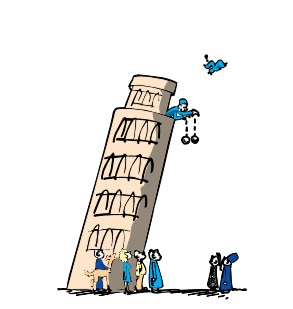
\includegraphics[width=0.6\textwidth]{fig/gali3.jpg}};
%%           \visible<2->{
%%           \node [rectangle,red,draw,text centered, rounded corners,fill=white] at (0.5,-0.5) (matter) {\small \bf{Matter}};
%%           \path [line,red] (matter)--(0.9,0.25);
%%           \node [rectangle,green,draw,text width=1.5cm,text centered, rounded corners,fill=white] at (2.5,-0.5) (antimatter) {\small \bf{Anti- matter}};
%%           \path [line,green] (antimatter)--(1.2,0.25);
%%          }
%%           \end{tikzpicture}
%%       \end{figure}
%%       \end{center}
%%   %%   \end{column}
%%   %% \end{columns}
%% \end{frame}

  
%% \begin{frame}{\centering The equivalence principle}
%%   \begin{columns}
%%     \begin{column}{0.39\textwidth}
%%         \begin{itemize}
%%         \item{Gravitational field = accelerated frame of reference}
%%         \item{Predicts: $\bar g= g$}
%%           \begin{itemize}
%%           \item{Never been tested before}
%%           \end{itemize}
%%         \item{Building block of general relativity}
%%           \begin{itemize}
%%             \uncover<2->{
%%             \item{Bending of light}
%%             \item{Red shift}
%%             }
%%           \end{itemize}
%%           \uncover<3->{\item{Matter-antimatter assymetry}}
%%           %\item{GPS}
%%       %\item{Test if the  weak equivalence principle holds also for antimatter}
%%       \end{itemize}
%%     \end{column}
%%     \begin{column}{0.65\textwidth}
%%       \begin{figure}
%%         \begin{tikzpicture}
%%           \node at (0,0){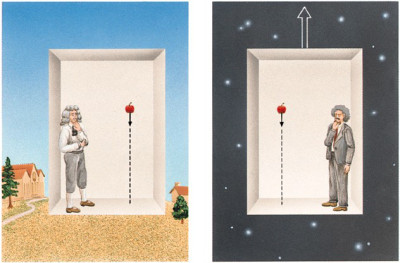
\includegraphics[width=\textwidth]{fig/elevator.jpg}};
%%           \node[scale=0.7,red] at (2.6,1.7){9.81~m/s$^2$};
%%          \end{tikzpicture}
%%       \end{figure}
%%     \end{column}
%%   \end{columns}
%%   \end{frame}
%% %\vskip 1cm

%% %\begin{block}{Examples}
  
%% %\end{block}

\begin{frame}{\centering A classical moiré deflectometer}
  \begin{center}
    \tikzstyle{line} = [draw, ultra thick,-latex]
    \tikzstyle{light} = [draw,color=gray]
    \tikzstyle{lineP} = [draw, ultra thick]
    \tikzstyle{block} = [rectangle, draw, fill=blue, 
      text width=6.0cm, text centered, rounded corners, minimum height=1em]

    %% \begin{columns}
    %%   \begin{column}{0.4\textwidth}
    %%     \begin{itemize}
    %%     \item Measure the gravitational accelration of antimatter
  %%     \item Test weak equivalence principle
  %%     \end{itemize}
  %%    \end{column}
  %%   \begin{column}{0.8\textwidth}
  \begin{tikzpicture}
    %\node at (0,0) {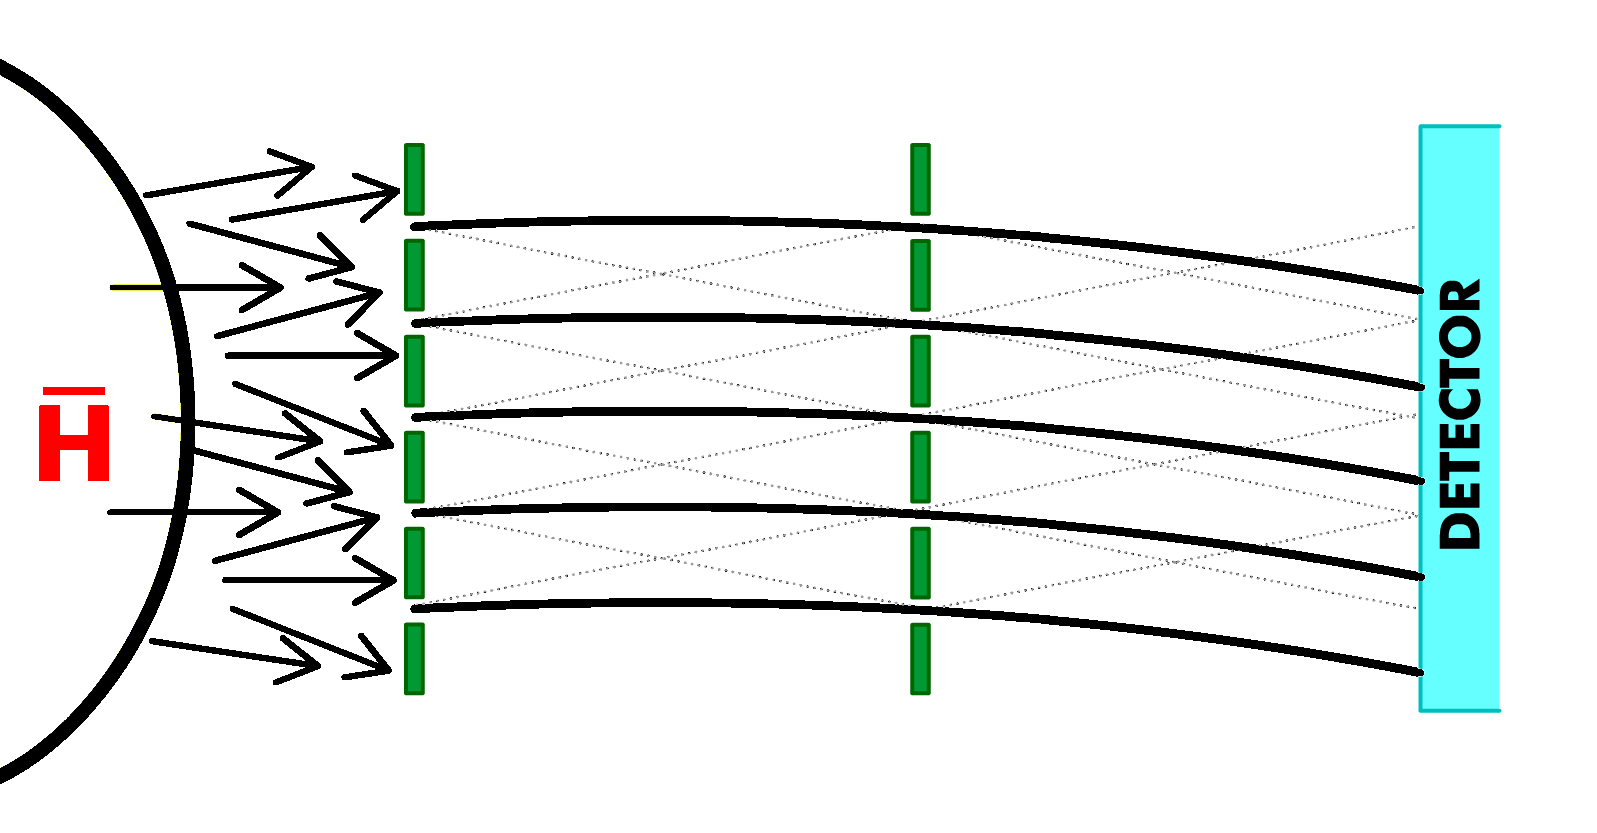
\includegraphics[width=\textwidth]{fig/moire.png}};

    %% \draw [decorate,decoration={brace,amplitude=10pt},rotate=0]
    %% (4.0,-2.3) -- (-2.5,-2.3) node [xshift=3.25cm,yshift=-0.6cm] {\textbf{1~m}};
    %% \draw [decorate,decoration={brace,amplitude=5pt},rotate=90]
    %% (0.5,-0.9) -- (-0.15,-0.9) node [xshift=0.8cm,yshift=0.3cm] {\bf{50~$\boldsymbol{\mu}$m}};

    \path [lineP] (0,0)--(0,0.8);
    \path [lineP] (0,1)--(0,1.8);
    \path [lineP] (0,2)--(0,2.8);
    \path [lineP] (0,3)--(0,3.8);
    \path [lineP] (0,4)--(0,4.8);
    \path [lineP] (0,5)--(0,5.8);
    

    \path [lineP] (4,0)--(4,0.8);
    \path [lineP] (4,1)--(4,1.8);
    \path [lineP] (4,2)--(4,2.8);
    \path [lineP] (4,3)--(4,3.8);
    \path [lineP] (4,4)--(4,4.8);
    \path [lineP] (4,5)--(4,5.8);


    \path [light] (0,-0.1)--(4,0.4);
    \path [light] (0,-0.1)--(8,1.9);
    \path [light] (0,-0.1)--(4,2.4);
    \path [light] (0,-0.1)--(8,3.9);
    \path [light] (0,-0.1)--(4,4.4);
    \path [light] (0,-0.1)--(8,5.9);  
    \path [light] (0,-0.1)--(4,5.4);

    \path [light] (0,0.9)--(4,0.4);
    \path [light] (0,0.9)--(8,0.9);
    \path [light] (0,0.9)--(4,1.4);
    \path [light] (0,0.9)--(8,2.9);
    \path [light] (0,0.9)--(4,2.4);   
    \path [light] (0,0.9)--(4,3.4);
    \path [light] (0,0.9)--(8,4.9);
    \path [light] (0,0.9)--(4,5.4);
    \path [light] (0,0.9)--(4,4.4);
    


    \path [light] (0,1.9)--(8,-0.1);
    \path [light] (0,1.9)--(4,0.4);
    \path [light] (0,1.9)--(8,1.9);
    \path [light] (0,1.9)--(4,2.4);
    \path [light] (0,1.9)--(8,3.9);
    \path [light] (0,1.9)--(4,4.4);
    \path [light] (0,1.9)--(8,5.9);

    \path [light] (0,1.9)--(4,1.4);
    \path [light] (0,1.9)--(4,3.4);
    \path [light] (0,1.9)--(4,5.4);
  

    
    \path [light] (0,2.9)--(4,0.4);
    \path [light] (0,2.9)--(8,0.9);
    \path [light] (0,2.9)--(4,1.4);
    \path [light] (0,2.9)--(8,2.9);
    \path [light] (0,2.9)--(4,3.4);
    \path [light] (0,2.9)--(8,4.9);
    \path [light] (0,2.9)--(4,5.4);

    \path [light] (0,2.9)--(4,2.4);
    \path [light] (0,2.9)--(4,4.4);


    \path [light] (0,3.9)--(8,-0.1);
    \path [light] (0,3.9)--(4,0.4);
    \path [light] (0,3.9)--(8,1.9);
    \path [light] (0,3.9)--(4,2.4);
    \path [light] (0,3.9)--(8,3.9);
    \path [light] (0,3.9)--(4,4.4);
    \path [light] (0,3.9)--(8,5.9);

    \path [light] (0,3.9)--(4,1.4);
    \path [light] (0,3.9)--(4,3.4);
    \path [light] (0,3.9)--(4,5.4);


    \path [light] (0,4.9)--(4,0.4);
    \path [light] (0,4.9)--(8,0.9);
    \path [light] (0,4.9)--(4,1.4);
    \path [light] (0,4.9)--(8,2.9);
    \path [light] (0,4.9)--(4,3.4);
    \path [light] (0,4.9)--(8,4.9);
    \path [light] (0,4.9)--(4,5.4);

    \path [light] (0,4.9)--(4,2.4);
    \path [light] (0,4.9)--(4,4.4);



    \path [light] (0,5.9)--(8,-0.1);
    \path [light] (0,5.9)--(4,0.4);
    \path [light] (0,5.9)--(8,1.9);
    \path [light] (0,5.9)--(4,2.4);
    \path [light] (0,5.9)--(8,3.9);
    \path [light] (0,5.9)--(4,4.4);

    \path [light] (0,5.9)--(4,1.4);
    \path [light] (0,5.9)--(4,3.4);
    \path [light] (0,5.9)--(4,5.4);

    \draw[domain=0:8,smooth] plot (\x,{5.9+0.2*\x-0.05*\x*\x});


    \draw[domain=-1:8,smooth,ultra thick, red] plot (\x,{2.9+0.05*\x-0.01*\x*\x});

    \draw[domain=-1:8,smooth,ultra thick, red] plot (\x,{2.9-0.2*\x-0.01*\x*\x});


    \draw[domain=-1:8,smooth,ultra thick, red] plot (\x,{2.9+0.3*\x-0.01*\x*\x});

    \node[draw,ultra thick, circle,color=red, fill=white, inner sep=0pt,minimum size=25pt] (b) at (-2,2) {$\bar H$};
    %\draw[ultra thick,red] (1,2.3) circle (0.3cm);

    %\path [draw,ultra thick,red](-1,1.4)parabola bend (4,2.9) (8,3.7);
    %\path [draw,ultra thick,red](-1,1.7)parabola through(1,1)(8,3.7);
    
    %\path [draw,ultra thick,red](0,2.9)parabola bend (3.9,4.4)(4,4.4);

    \node [block,rotate=90] at (8.2,2.9) {Detector};

    \visible<3->{
    \node[star, star points=5, minimum width=0.1cm,inner sep=1.8pt,anchor=outer point 3,star point ratio=5.25, fill=yellow, draw] at (7.65,-0.4) {};

    \node[star, star points=5, minimum width=0.1cm,inner sep=1.8pt,anchor=outer point 3,star point ratio=5.25, fill=yellow, draw] at (7.65,0.55) {};

    \node[star, star points=5, minimum width=0.1cm,inner sep=1.8pt,anchor=outer point 3,star point ratio=5.25, fill=yellow, draw] at (7.65,1.5) {};

    \node[star, star points=5, minimum width=0.1cm,inner sep=1.8pt,anchor=outer point 3,star point ratio=5.25, fill=yellow, draw] at (7.65,2.45) {};

    \node[star, star points=5, minimum width=0.1cm,inner sep=1.8pt,anchor=outer point 3,star point ratio=5.25, fill=yellow, draw] at (7.65,3.4) {};

    \node[star, star points=5, minimum width=0.1cm,inner sep=1.8pt,anchor=outer point 3,star point ratio=5.25, fill=yellow, draw] at (7.65,4.4) {};

    \node[star, star points=5, minimum width=0.1cm,inner sep=1.8pt,anchor=outer point 3,star point ratio=5.25, fill=yellow, draw] at (7.65,5.4) {};
}
    
    %\node[star, star points=5, minimum width=0.1cm,inner sep=1.8pt,anchor=outer point 3,star point ratio=5.25, fill=yellow, draw] at (7.4,3.35) {};

    
    %% \node[star, star points=5, minimum width=0.1cm,inner sep=1.8pt,anchor=outer point 3,star point ratio=5.25, fill=yellow, draw] at (8,0.4) {};
    %% \node[star, star points=5, minimum width=0.1cm,inner sep=1.8pt,anchor=outer point 3,star point ratio=5.25, fill=yellow, draw] at (8,0.9) {};
    %% \node[star, star points=5, minimum width=0.1cm,inner sep=1.8pt,anchor=outer point 3,star point ratio=5.25, fill=yellow, draw] at (8,1.4) {};
    %% \node[star, star points=5, minimum width=0.1cm,inner sep=1.8pt,anchor=outer point 3,star point ratio=5.25, fill=yellow, draw] at (8,1.9) {};
    %% \node[star, star points=5, minimum width=0.1cm,inner sep=1.8pt,anchor=outer point 3,star point ratio=5.25, fill=yellow, draw] at (8,2.4) {};
    %% \node[star, star points=5, minimum width=0.1cm,inner sep=1.8pt,anchor=outer point 3,star point ratio=5.25, fill=yellow, draw] at (8,2.9) {};
    %% \node[star, star points=5, minimum width=0.1cm,inner sep=1.8pt,anchor=outer point 3,star point ratio=5.25, fill=yellow, draw] at (8,3.4) {};
    %% \node[star, star points=5, minimum width=0.1cm,inner sep=1.8pt,anchor=outer point 3,star point ratio=5.25, fill=yellow, draw] at (8,3.9) {};
    %% \node[star, star points=5, minimum width=0.1cm,inner sep=1.8pt,anchor=outer point 3,star point ratio=5.25, fill=yellow, draw] at (8,4.4) {};
    %% \node[star, star points=5, minimum width=0.1cm,inner sep=1.8pt,anchor=outer point 3,star point ratio=5.25, fill=yellow, draw] at (8,4.9) {};
    %% \node[star, star points=5, minimum width=0.1cm,inner sep=1.8pt,anchor=outer point 3,star point ratio=5.25, fill=yellow, draw] at (8,5.4) {};
    %% \node[star, star points=5, minimum width=0.1cm,inner sep=1.8pt,anchor=outer point 3,star point ratio=5.25, fill=yellow, draw] at (8,5.9) {};
  
    

    %\node[star,fill=red,minimum width=0.2cm] at (0,0) {};
    %\visible <2> {\node at (6,0) {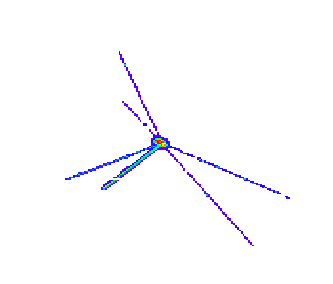
\includegraphics[width=0.4\textwidth]{fig/antiprotonExTest.png}};}
    %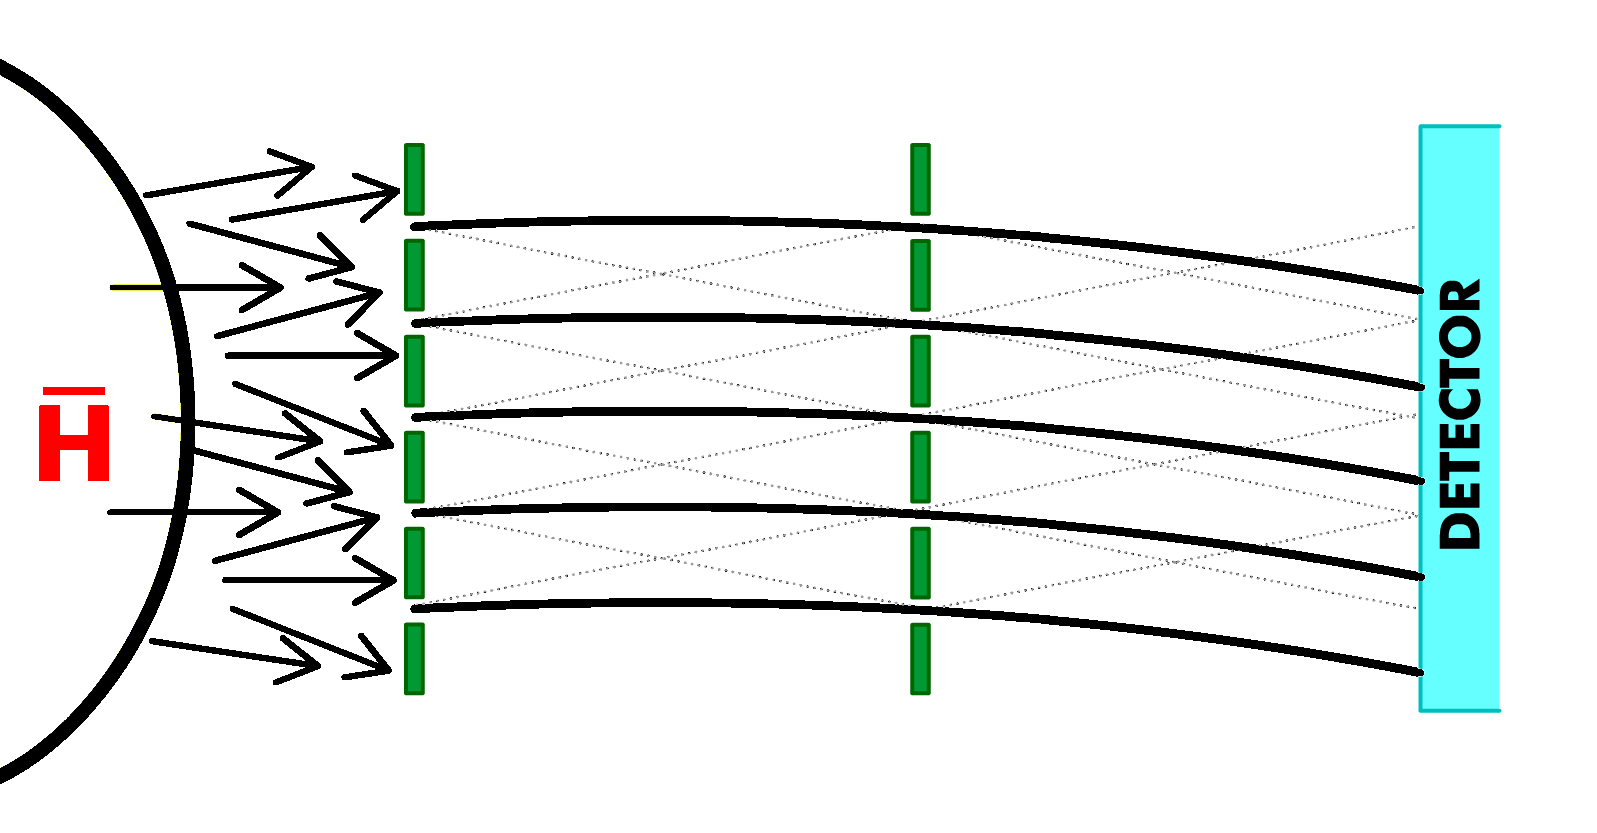
\includegraphics[width=0.8\textwidth]{fig/moire.jpg}
  \end{tikzpicture}
  %%   \end{column}
  %% \end{columns}
  \end{center}
\end{frame}

%% \begin{frame}{\centering Requirements for the detector}  
%%   %% \begin{columns}
%%   %%   \begin{column}{0.4\textwidth}
%%   \begin{itemize}
%%     \item{Tag antihydrogen}
%%       \uncover<2->{
%%         \begin{itemize}
%%         \item{Fragments from annihilations outside the detector}
%% %        \item{Trade off between tagging efficiency and purity of sample}
%%         \end{itemize}
%%       }
%%   \item{Measure time of flight}
%%     \uncover<3->{\begin{itemize}
%%       \item{Energy of antihydrogen beam will not be completely uniform}
%%       \item{Transit time through the moirè deflectometer is around 2ms}
%%       \end{itemize}
%%       }
%%   \item{Reconstruct the annihilation point}
%%     \uncover<4->{\begin{itemize}
%%       \item{The periodicity of the moire deflectometer is around 50~$\mu$m}
%%       \item{Vertical fall around 10~$\mu$m}
%%       \item{Around 10~$\mu$m resolution needed to achieve 1\% precision on $\bar g$}
%%       \end{itemize}
%%     }
%%     \uncover<5->{
%%     \item{Does a detector fullfilling these requirements already exist?}
%%       }
%%   \end{itemize}
%%   %%    \end{column}
%%   %%   \begin{column}{0.8\textwidth}
%%   %\begin{figure}
%%   %  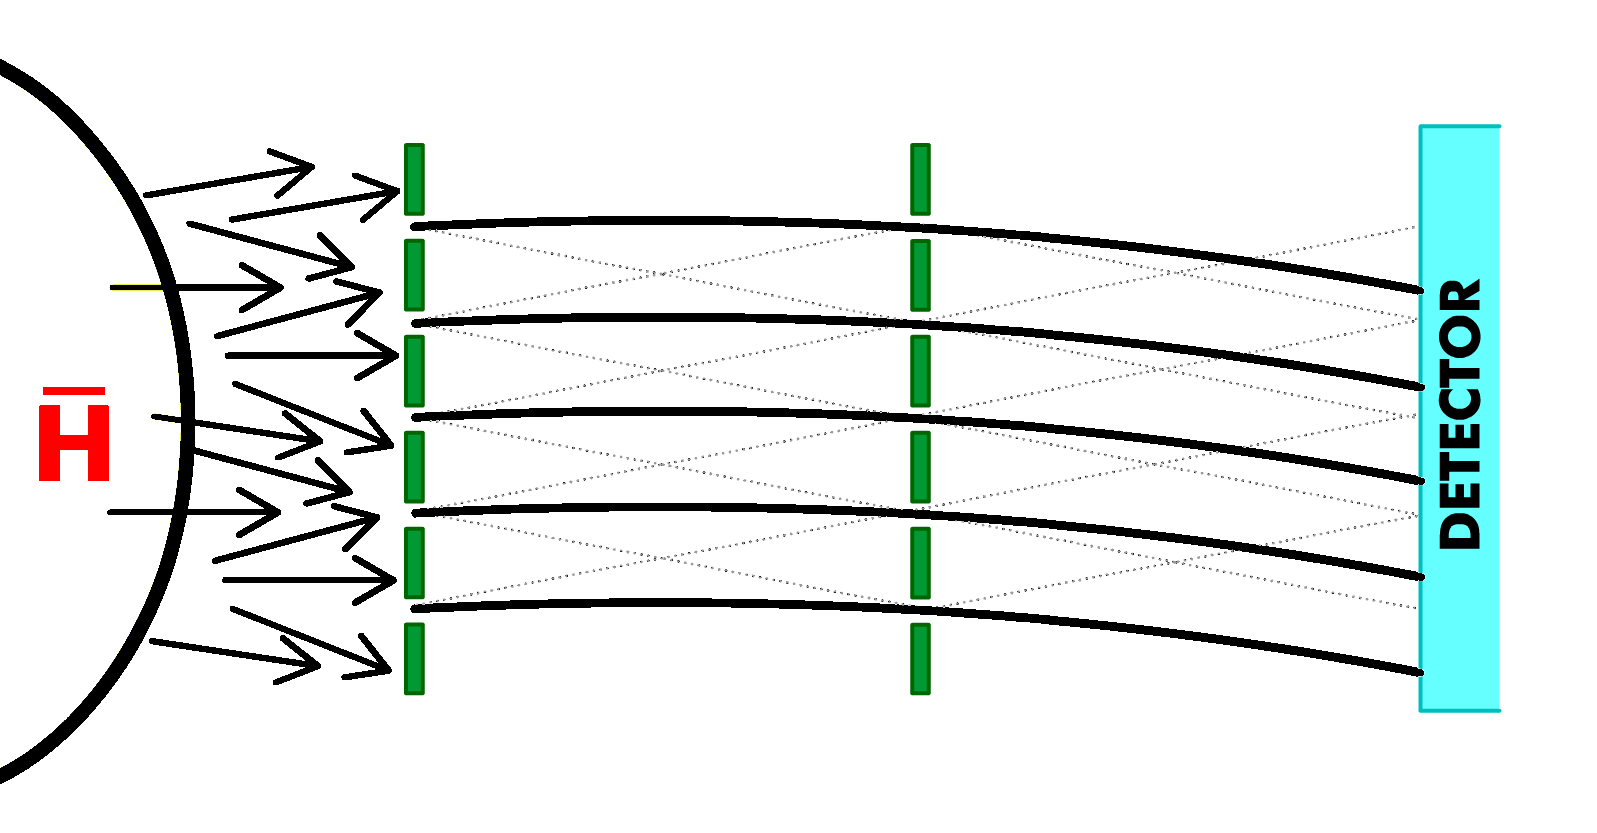
\includegraphics[width=0.8\textwidth]{fig/moire.png}
%%   %\end{figure}
%%   %%   \end{column}
%%   %% \end{columns}
%% \end{frame}


%% \begin{frame}{\centering Silicon pixel detector using the Timepix3 readout system}
%%   \begin{columns}
%%     \begin{column}{0.5\textwidth}
%%       \begin{itemize}
%%       \item{55~$\mu$m$\times$55~$\mu$m pixels}
%%       \item{Measure both time of arrival and deposited energy}
%%       \item{Time resolution 1--2~ns}
%%       \item{670~$\mu$m thick}
%%       \item{Expose the Timepix3 detector to antiprotons as the annihilation process is the same}
%%       \end{itemize}
%%      \end{column}
%%     \begin{column}{0.5\textwidth}
%%       \begin{tikzpicture}
%%         \node at (0,0) {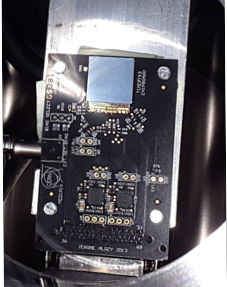
\includegraphics[width=0.8\textwidth]{fig/MountedTimepix.png}};
%%         \visible<2>{\node at (0,0) [red,scale=8]{?};}
%%         \end{tikzpicture}
%%     \end{column}
%%   \end{columns}
%%  \end{frame}

%% \begin{frame}{\centering GRACE beamline}
%%   \vspace{0.025cm}
%%   \only<1>{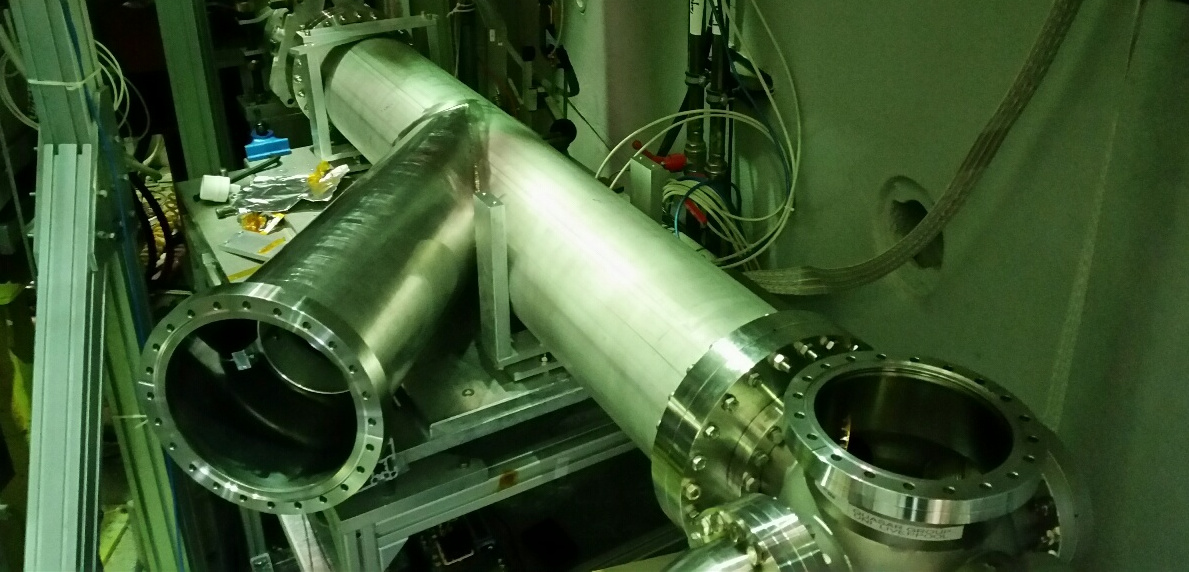
\includegraphics[width=\textwidth]{fig/GRACEReal.jpg}}
%% %  \only<2>{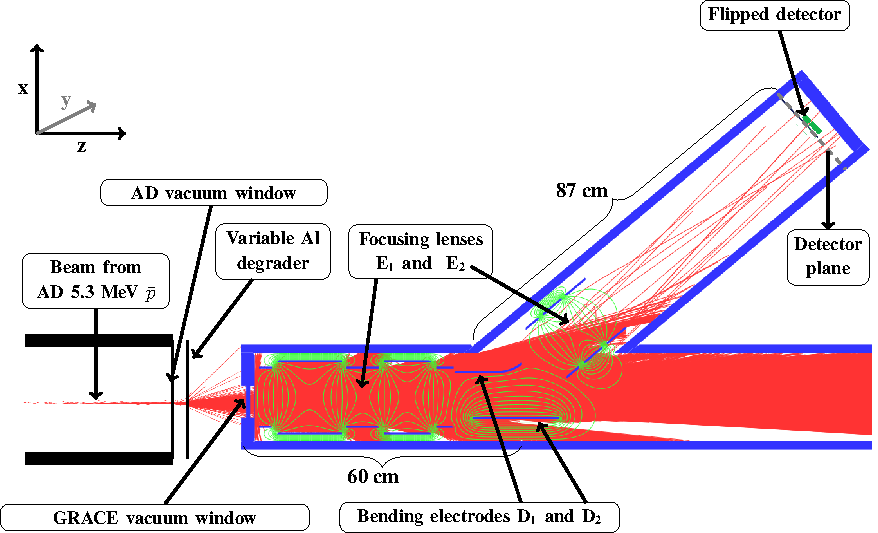
\includegraphics[width=\textwidth]{fig/thesis-figure1.pdf}}
%% \end{frame}


%% \begin{frame}{\centering GRACE in standard setting}
%%   \vspace{0.025cm}
%%   \only<1>{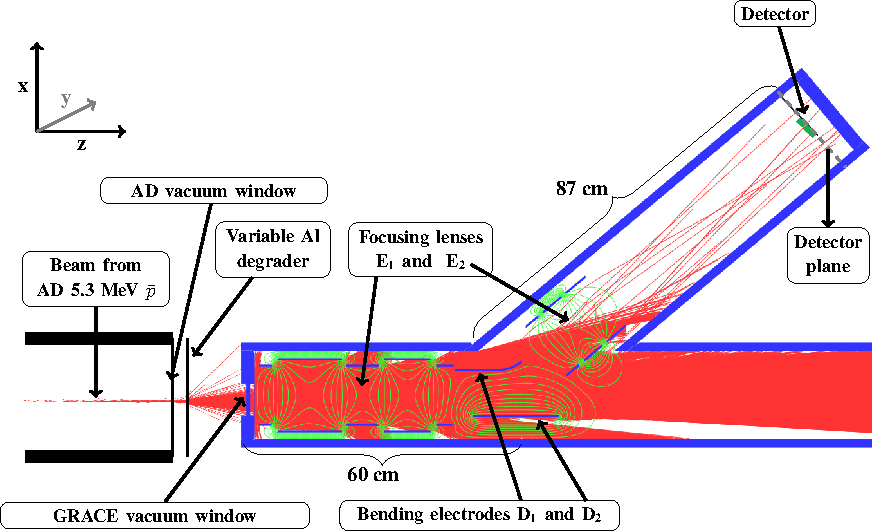
\includegraphics[width=\textwidth]{fig/thesis-figure0.pdf}}
%% %  \only<2>{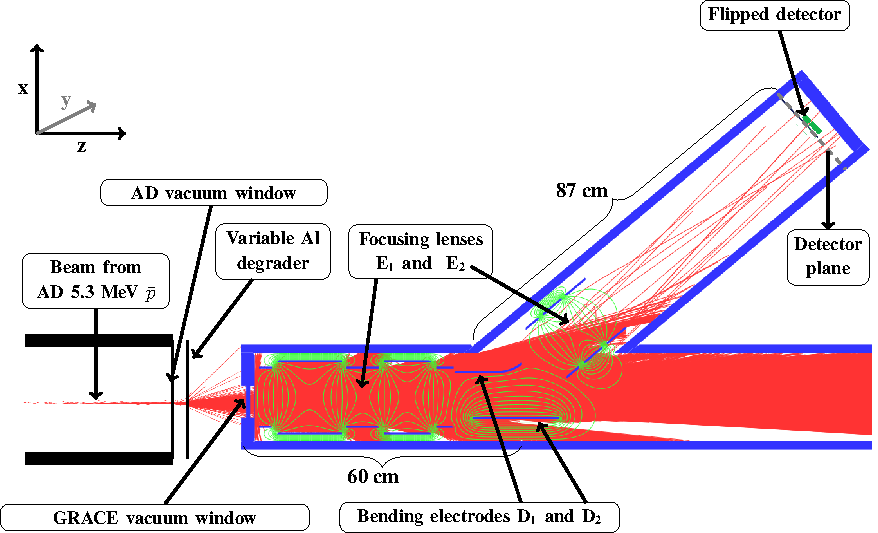
\includegraphics[width=\textwidth]{fig/thesis-figure1.pdf}}
%% \end{frame}



%% \begin{frame}{\centering GRACE for reference sample}
%%  % \only<1>{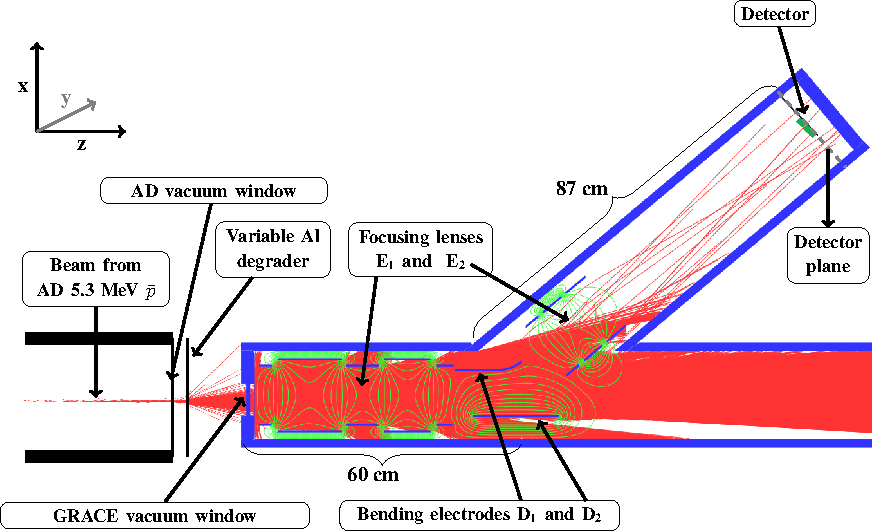
\includegraphics[width=\textwidth]{fig/thesis-figure0.pdf}}
%%   \only<1>{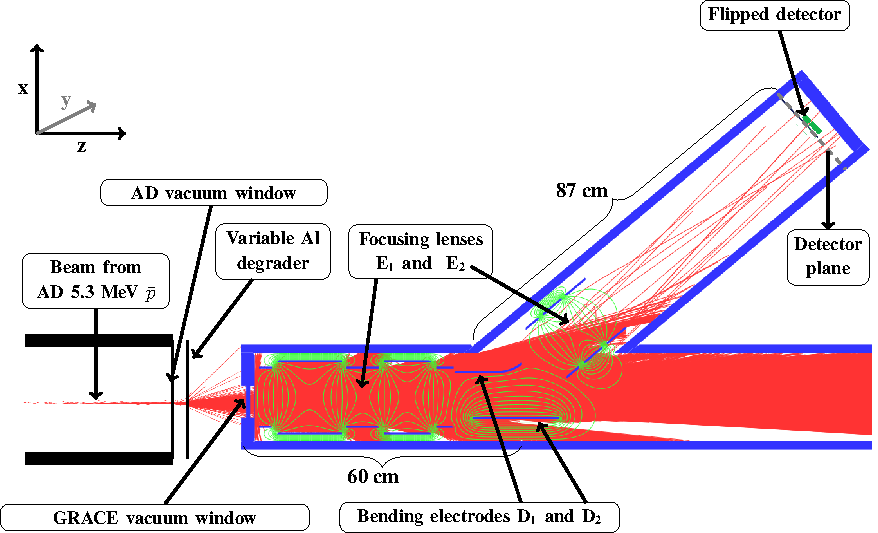
\includegraphics[width=\textwidth]{fig/thesis-figure1.pdf}}
%% \end{frame}



%% \begin{frame}{\centering Antiproton data}
%%   %\begin{center}
%%   \vspace{-0.5cm}
%%   \begin{center}
%%     \only<1>{
%%       \resizebox{11.3cm}{8.3cm}{%
%%          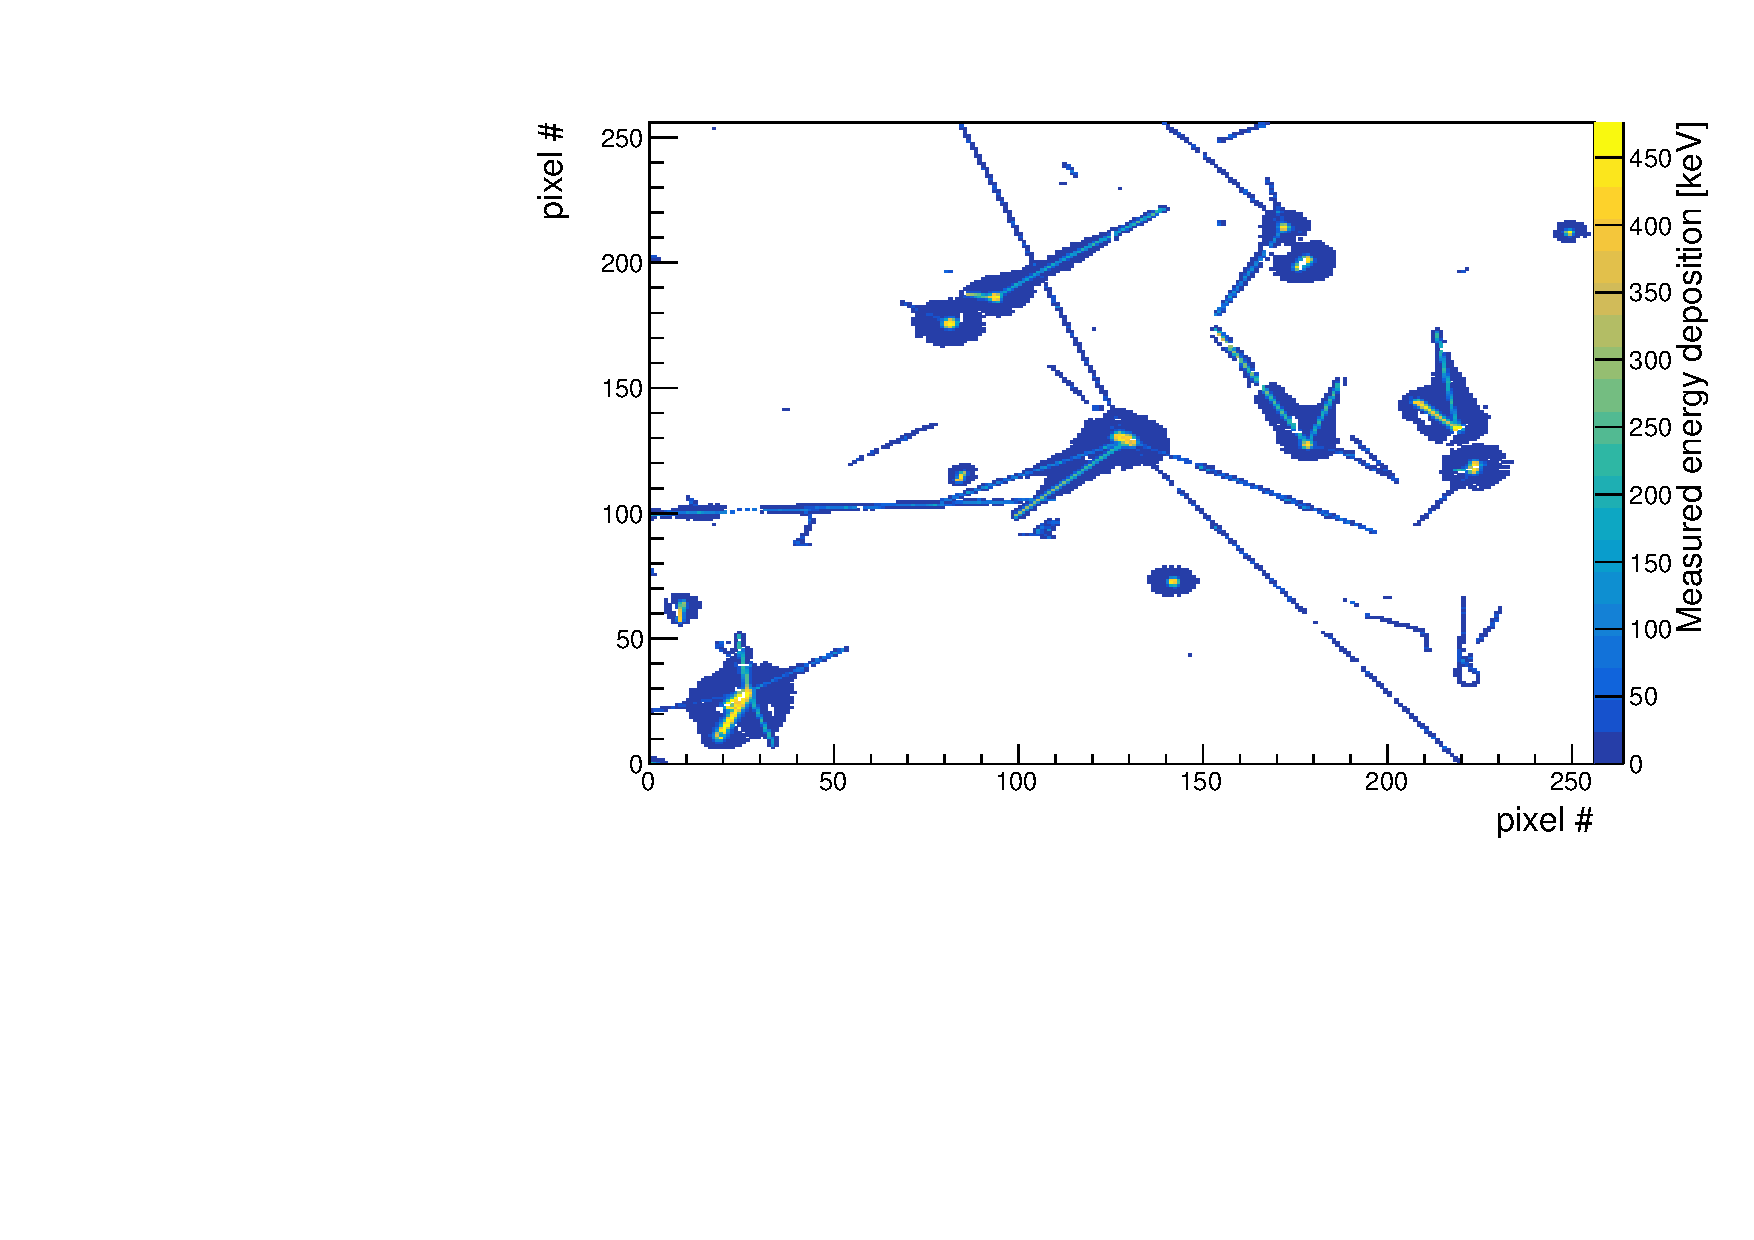
\includegraphics[width=5.0in]{fig/fullFrameUncleaned.pdf}
%%        }
%%        }
%%     \only<2>{
%%       \resizebox{11.3cm}{8.3cm}{%
%%     \begin{tikzpicture}
%%     \node[inner sep=0pt] (russell) at (0,0){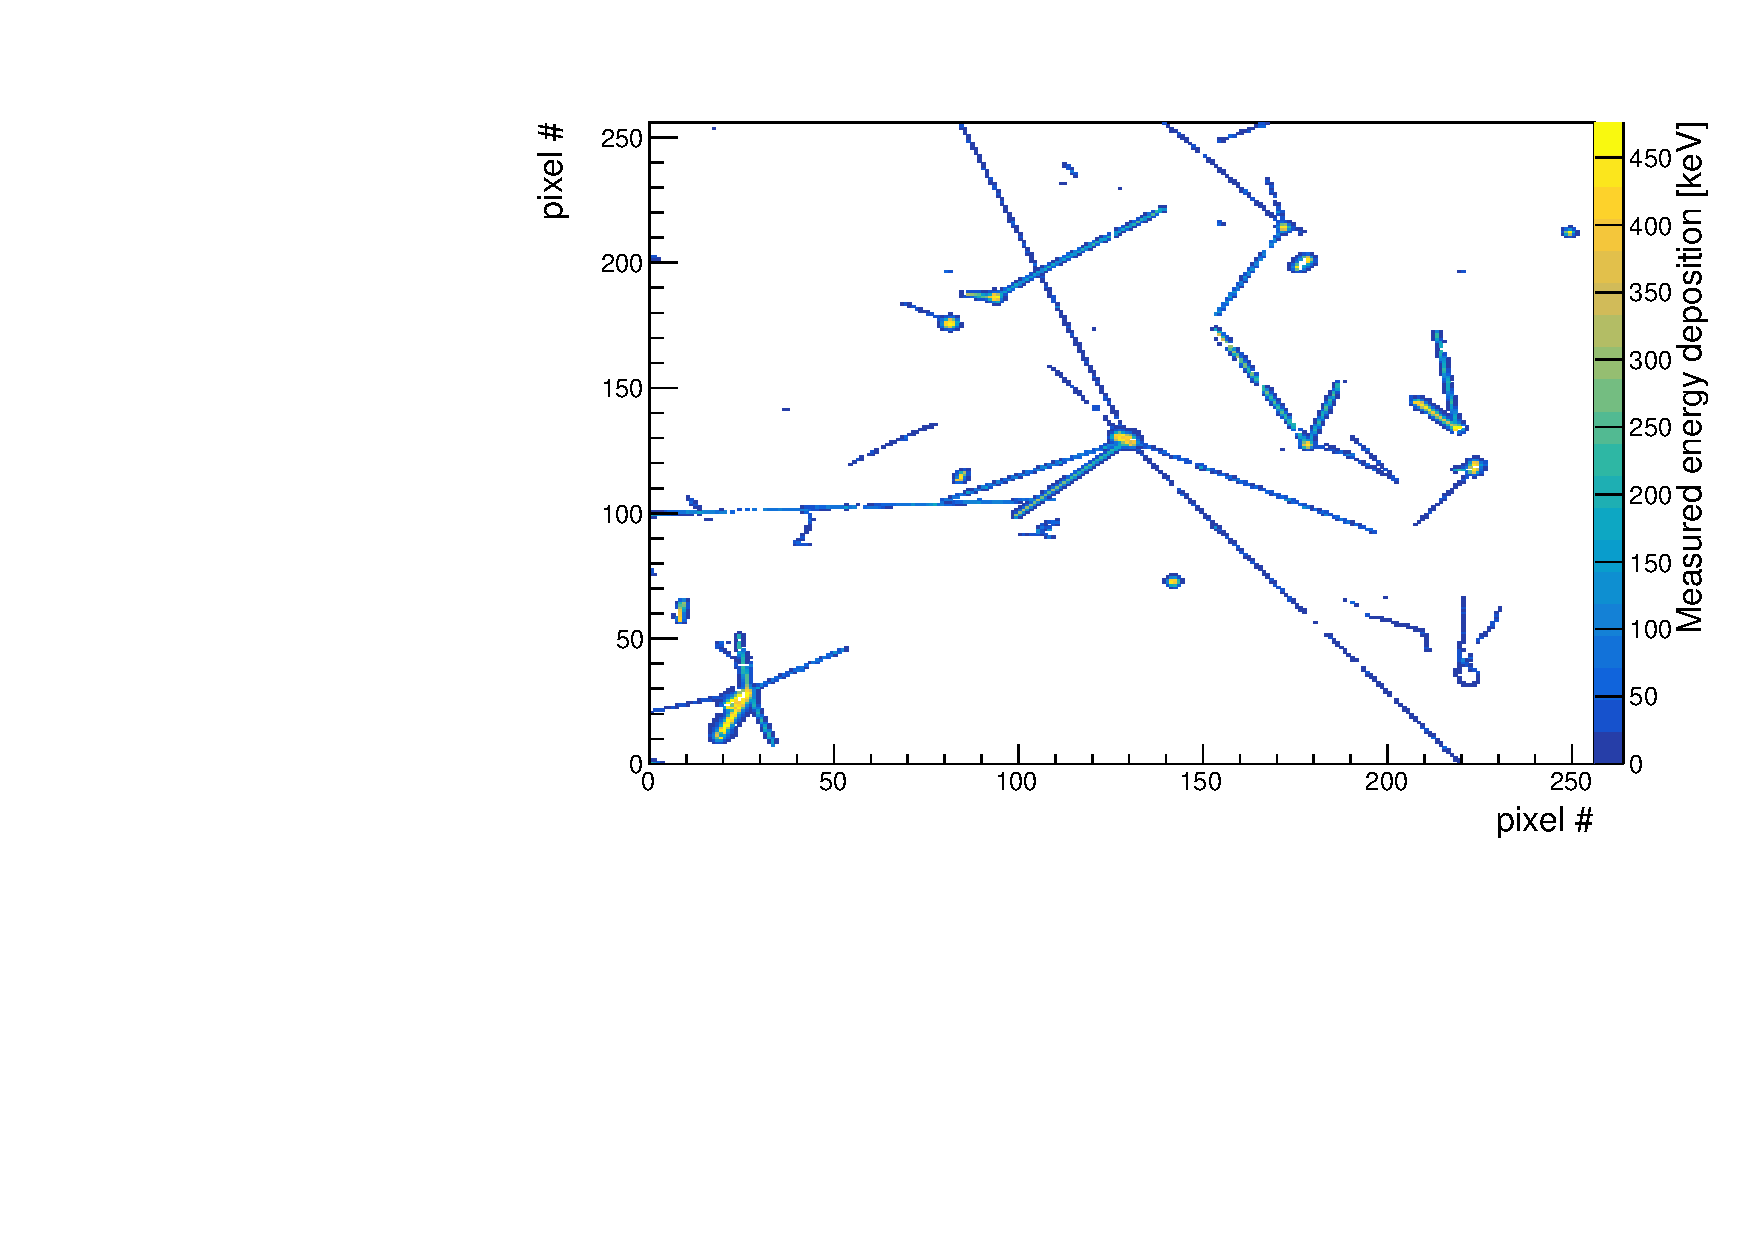
\includegraphics[width=5.0in]{fig/fullFrame.pdf}};
%%     %\draw [<-,black, thick] (-2.2,-1.6) to (-0.7,-2.0);
%%     %\draw [<-,black, thick] (0.03,-0.13) to (-0.5,-1.6);
%%     \node [rectangle,draw,text centered, rounded corners,text width=1.8cm,fill=white] at (-0.0,-2.7) (ann){\small Clear \\ annihilations };
%%     %\draw [<-,black, thick] (-1.2,0.9) to (-1.55,2.0);
%%     %\draw [<-,black, thick] (-0.9,1.1) to (-1.55,2.0);
%%     \node [draw,text width=2.0cm,text centered, rounded corners,fill=white] at (-3.45,2.9) (pani){\small Annihilation \\ candidates  };
%%     %\draw [<-,black, thick] (-1.7,0.1) to (-2.3,1.0);
%%     %\node [rectangle,text width=2.28cm,draw,text centered, rounded corners,fill=white,execute at begin node=\setlength{\baselineskip}{0.4em}] at (-4.5,0.6) (prob2) {\small Zero \\ \small prongs};
%%     %\node [rectangle,draw,text width=2.28cm,text centered, rounded corners,fill=white,execute at begin node=\setlength{\baselineskip}{0.4em}] at (3.4,2.95) (prob1) {\small Zero \\ \small prongs };
%%     \node [rectangle,text width=1.0cm,draw,text centered, rounded corners,fill=white] at (-4.5,0.6) (prob2) {\small Zero \\ \small prongs};
%%     \node [rectangle,draw,text width=1.0cm,text centered, rounded corners,fill=white] at (3.4,2.95) (prob1) {\small Zero \\ \small prongs };

%%     \path [line] (prob2)--(-2.5,0.05);
%%     \path [line] (prob1)--(2,2);
%%     \path  [line] (pani)--(-2.0,1.4);
%%     \path  [line] (pani)--(-1.6,1.7);
%%     \path  [line] (ann)--(-3.5,-2.55);
%%     \path  [line] (ann)--(0,-0.15);
%%     \end{tikzpicture}
%%     }
%%     }
%%     \end{center}
%%   %\end{center}
%%   %\hspace{10cm}
%% \end{frame}
%% \begin{frame}
%%   \scalebox{0.6}{{
  \vspace{-1cm}
  \hspace{-1.5cm}
  % Define block styles
  \tikzstyle{block} = [rectangle, draw, fill=blue!90!green!90!black!20, 
    text width=2.7cm, text centered, rounded corners, minimum height=1em]
  \tikzstyle{mainBlock} = [rectangle, draw, fill=green!20, 
  text width=3.0cm,ultra thick, text centered, rounded corners, minimum height=1cm]
  \tikzstyle{line} = [draw, ultra thick,-latex]
  \tikzstyle{lineP} = [draw, ultra thick]
  \tikzstyle{cloud} = [draw ,fill=red!20,text width=2.6cm,minimum height=4em,text centered]
  \tikzstyle{problem} = [rectangle, draw, fill=yellow!90, 
    text width=2.5cm, text centered, rounded corners, minimum height=1em]

  %\tikzstyle{problem} = [star, star points=5, minimum width=0.0cm,inner sep=0.1pt,anchor=outer point 10,star point ratio=2.0, fill=yellow,text width=1cm, draw]
  %\begin{center}
    \begin{tikzpicture}
      %\vspace{-2cm}
      \visible<1->{
      \node [mainBlock](data) {\large Raw data from Timepix3};
      \node [mainBlock,left of =data,xshift=10cm](simu) {\large Monte Carlo generated annihilations from FLUKA};
      \node [mainBlock,below of =data,yshift=-2cm](dataP) {\large Processed data};
      \node [mainBlock,below of =simu,yshift=-2cm](simuP) {\large Simulated data};
      \path [line] (data)--(dataP) node[left,align=center,yshift=1.5cm,xshift=2.2cm] {~~-Clustering\\-Cleaning};
      \path [line] (simu)--(simuP) node[left,align=right,yshift=1.5cm,xshift=-0.2cm] {Detector response};
      }
      
      \visible<2,3,4>{\path [lineP] (dataP)--(simuP) node[above,align=right,yshift=0cm,xshift=-4.5cm] {\huge?};
      }

      \visible<5->{\path [lineP] (dataP)--(simuP) node[above,align=right,yshift=0cm,xshift=-4.5cm] {\huge =};
        }
            %%  %\path [lineP] (simuP)--(Obs) node[above,align=right,yshift=0cm,xshift=-7.0cm] {};
      \visible<3->{
        \node [cloud,below of =simuP,yshift=-1.5cm,xshift=-4.5cm](Obs) {\large Observables};
      \node [mainBlock,below of =simuP,yshift=-3cm](ObsS) {\large
        %--Størrelse \\
        %--\\
        \begin{itemize}
        \item{Deposited energy}
        \item{Deposited energy in center}
        \item{Size}
        \item{Prongs}
        \end{itemize}
        };
      \node [mainBlock,below of =dataP,yshift=-3cm](ObsD) {\large
      \begin{itemize}
      \item{Deposited energy}
      \item{Deposited energy in center}
      \item{Size}
      \item{Prongs}
      \end{itemize}
      };
      \path [line] (Obs)--(ObsD); 
      \path [line] (Obs)--(ObsS); 
      \path [lineP] (simuP)--(Obs);
      \path [lineP] (dataP)--(Obs);
      \node [cloud,below of =ObsS,yshift=-1.5cm,xshift=-4.5cm](Sam) {\large Compare distributions};
      \path [line] (ObsS)--(Sam); 
      \path [line] (ObsD)--(Sam);
      
      }


      \visible<4>{
        \node [problem,left of=simu,xshift=3.0cm,yshift=-1.8cm,text width=2.8cm]{\large{Improve the response model}};
      }

      
      \visible<6->{\node [mainBlock,text width=5cm,below of =Sam,yshift=-1.5cm,xshift=0cm](Fin) {\large \begin{itemize}
        \item{Tag antiprotons}
        \item{Reconstruct annihilation point}
        \item{...}
        \end{itemize}
        };
        \path [line] (simuP)|-($(simuP)+(3cm,0cm)$) |- (Fin);
        \path [line] (dataP)-|($(dataP)+(-3cm,0cm)$) |- (Fin);
      }
      \visible<7->{
        \node [mainBlock,left of =simu,yshift=0cm,xshift=5cm](Sann) {\large Truth information};
        \node [mainBlock,below of=Sann,yshift=-13cm,xshift=0cm](Eva) {\large Evaluate methods};
        \path [line] (simu)--(Sann);
        \path [line] (Sann)--(Eva);
        %\path [line] (Fin)--($(Fin)+(0cm,0cm)$) |- (Eva);
        \path [line] (Fin)|-($(Fin)+(0cm,-2cm)$)|-(Eva);
      %
      %% \path [line] (ObsS)--(Sam); 
      %% \path [line] (ObsD)--(Sam); 
      }
      \visible<8>{
        \node [problem,left of=data,xshift=-2.1cm,yshift=0cm]{\large{Bad experimental conditions}};
      }

        \visible<10>{
        \node [problem,left of=simu,xshift=-2.1cm,yshift=0cm]{\large{Annihilation process not fully known}};
        }

         \visible<11>{
           \node [problem,left of=Eva,xshift=-0.5cm,yshift=1.2cm]{\large{Effect on final results}};
           }
         \visible<9>{
        \node [problem,above of=Sam,xshift=0.0cm,yshift=1cm]{\large{Data contains mixture of fragments and annihilations}};
        }

      
    \end{tikzpicture}
  %\end{center}
}

%%% Local Variables: 
%%% mode: latex
%%% TeX-master: "../../thesis.tex"
%%% End: 
}
%% \end{frame}




%% \begin{frame}{\centering Detector response model}
%%   \begin{columns}
%%     \begin{column}{0.45\textwidth}
%%       \begin{itemize}
%%       \item<1->{Raw energy depositions in small voxels (FLUKA)}
%%       \item<2->{Parametrized model for charge sharing including the plasma effect}
%%       \item<3->{Volcano effect}
%%       \item<4->{Suppressed pixels in the experimental set-up}
%%       \item<4->{Re-clustering}
%%       \end{itemize}
%%     \end{column}
%%     \begin{column}{0.55\textwidth}
%%       \begin{tikzpicture}
%%       \only<1>{\node at (0,0){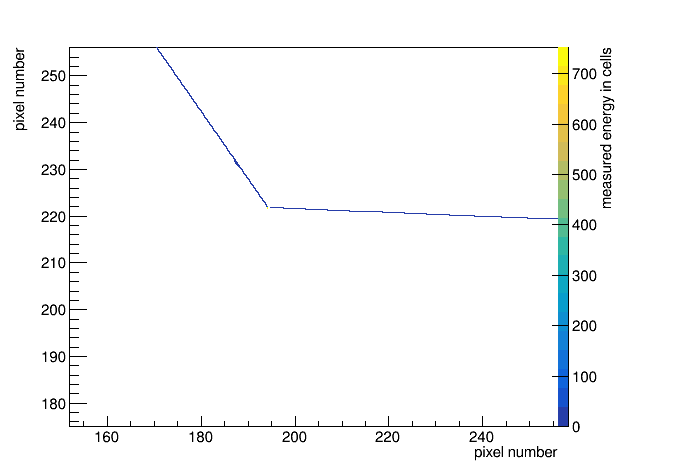
\includegraphics[width=2.55in]{fig/test/initial.png}}};
%%        \only<2>{\node at (0,0){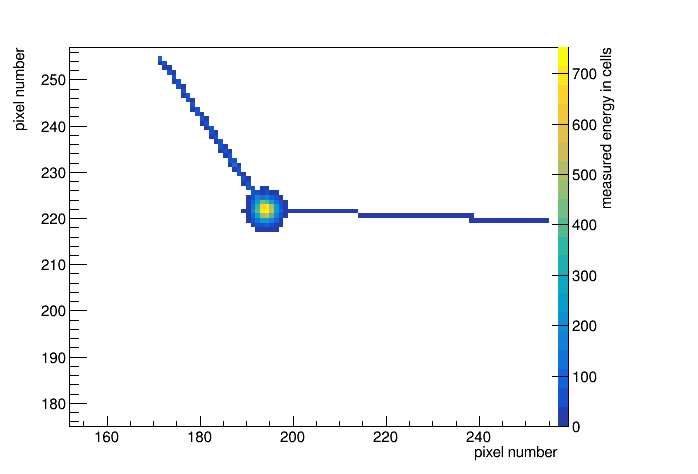
\includegraphics[width=2.55in]{fig/test/afterBlur.png}}};
%%       \only<3>{\node at (0,0){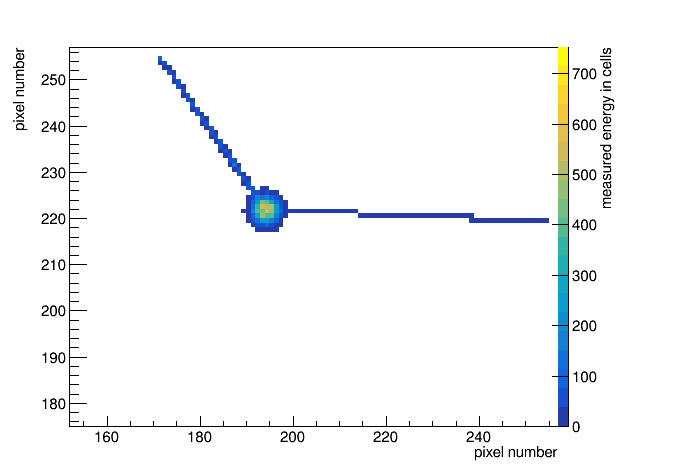
\includegraphics[width=2.55in]{fig/test/afterVolcano.png}}};
%%       \only<4>{\node at (0,0){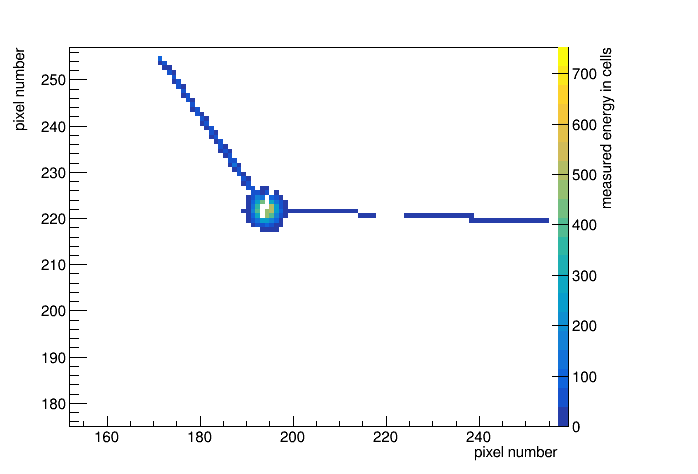
\includegraphics[width=2.55in]{fig/test/final.png}}};
%%       \end{tikzpicture}
%%     \end{column}
%%     \end{columns}
%% \end{frame}



%% \begin{frame}{\centering Analyse the data}
%%   \begin{columns}
%%     \begin{column}{0.5\textwidth}
%%       \begin{itemize}
%%       \item<1->{Clustering in time and space}
%%       \item<2->{Find center}
%%       \item<3->{Estimate annihilation point (mass center method)}
%%       \item<4->{Reomve center}
%%       \item<5->{Hough transform to identify prongs}
%%       \item<6->{Remove prong (star arms)}
%%       \item<7->{Find more prongs}
%%       \item<8->{Check for single tracks}
%%       \item<11>{Fit lines to the prongs and find intersection (vertex fitting method)}
%%       \end{itemize}
%%     \end{column}
%%     \begin{column}{0.55\textwidth}
%% %%       %%       test
%%       \begin{tikzpicture}
%%         \only<1,2,3>{\node at (0,0){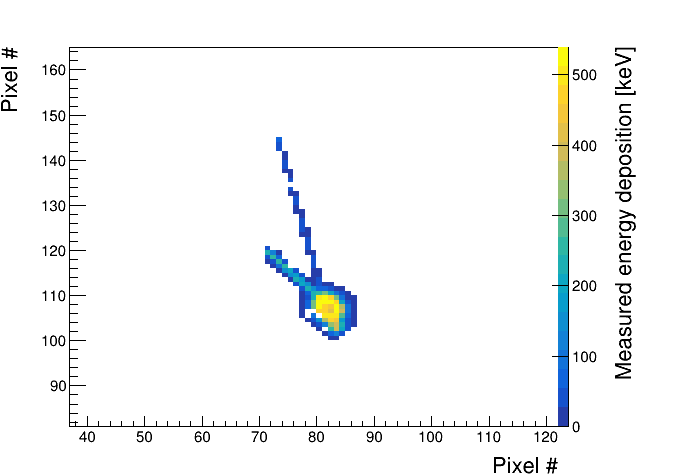
\includegraphics[width=2.55in]{fig/370.png}};}         \only<2,3>{\draw[orange,thick] (-0.27,-0.78) circle (0.24);}
%%         \only<3>{\draw[black,thick,fill=black] (-0.22,-0.72) circle (0.03);}
%%         \only<4,5>{\node at (0,0){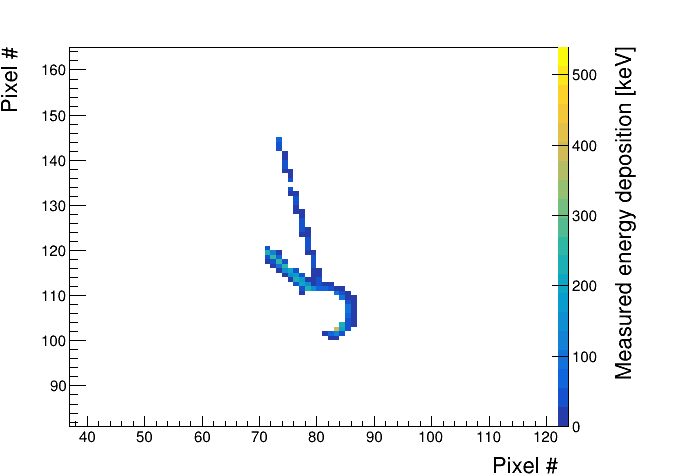
\includegraphics[width=2.55in]{fig/371.png}};}
%%         \only<6>{\node at (0,0){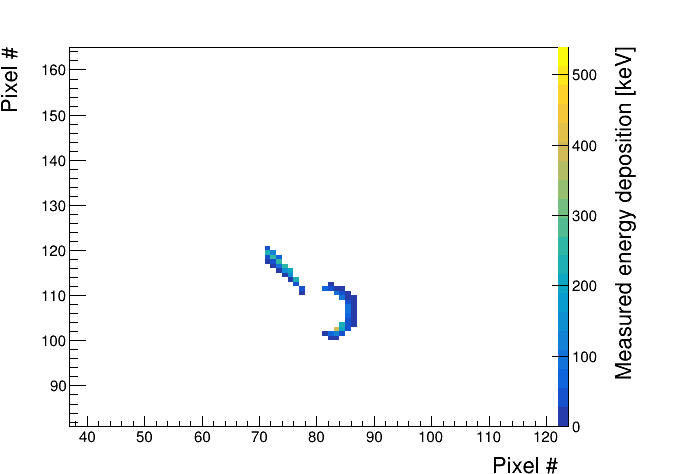
\includegraphics[width=2.55in]{fig/372.png}};}
%%         \only<7>{\node at (0,0){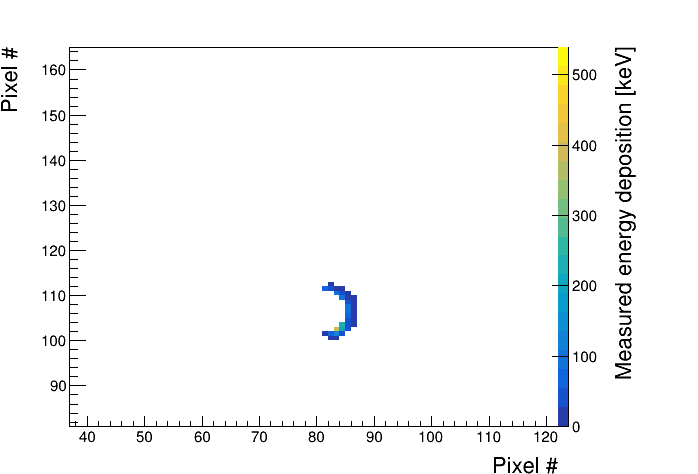
\includegraphics[width=2.55in]{fig/373.png}};}
%%            %% %%
%%         \only<8,9>{\node at (0,0){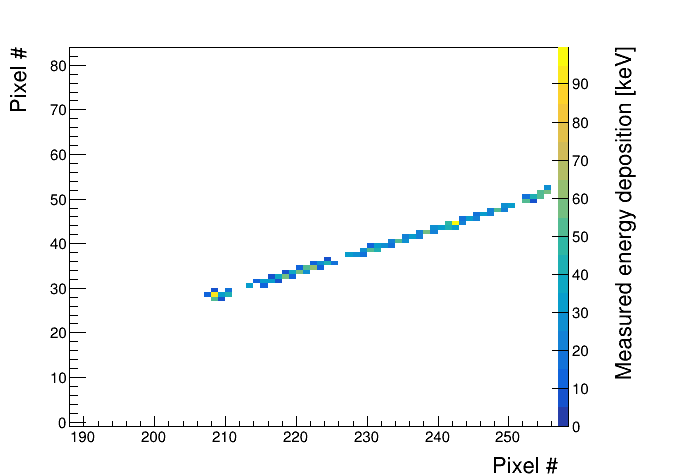
\includegraphics[width=2.55in]{fig/1060.png}};}
%%         \only<9>{\draw [thick,red](-2.8,-1)--(2.1,0.45);}
      
%%         \only<10>{\node at (0,0){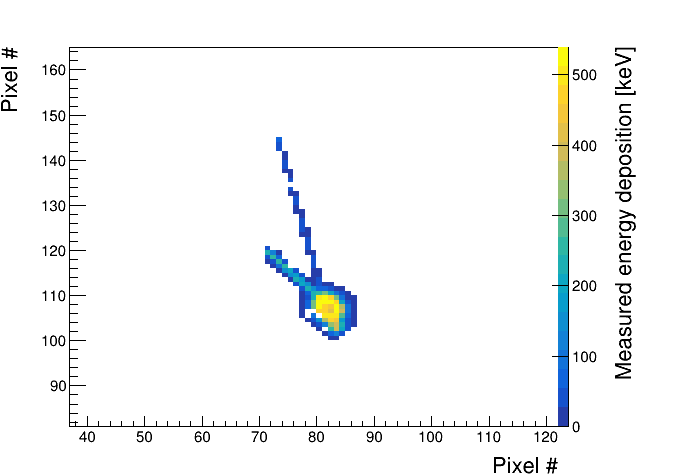
\includegraphics[width=2.55in]{fig/370.png}};}
%%         \only<10>{\draw [thick,red](-1.8,1.9)--(0.5,-1.9);}
%% %%    
%% %%         %% \only<9>{\node at (0,0){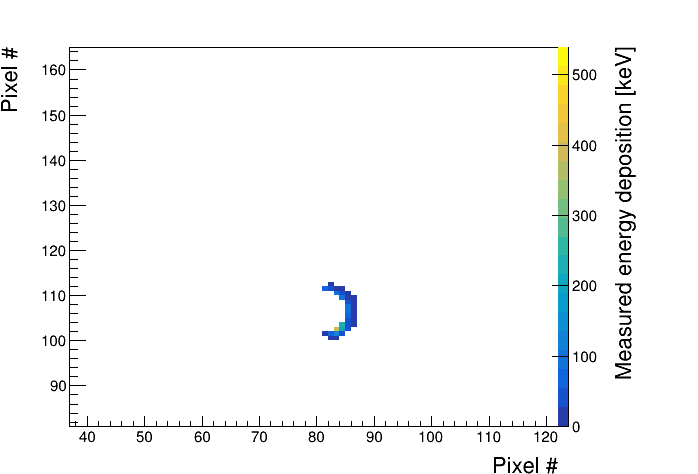
\includegraphics[width=2.55in]{fig/373.png}};}
%% \only<11>{\node at (0,0){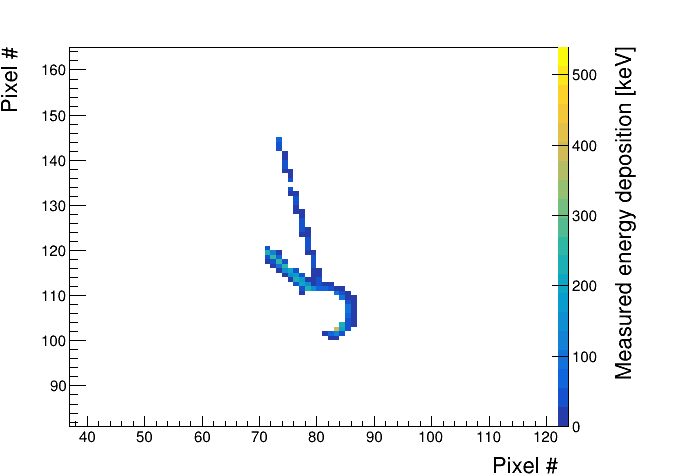
\includegraphics[width=2.55in]{fig/371.png}};}
%% \only<11>{\draw [thick,green](-2.8,1.6)--(0.7,-1.45);}
%% \only<11>{\draw [thick,green](-0.95,2)--(-0.0,-1.45);}
%%       \end{tikzpicture}
%%     \end{column}
%%   \end{columns}
%% \end{frame}



%% \begin{frame}{\centering Verification of the simulation}
%%   \only<1>{\begin{block}{\centering Cluster energy}
%%     \centering
%%     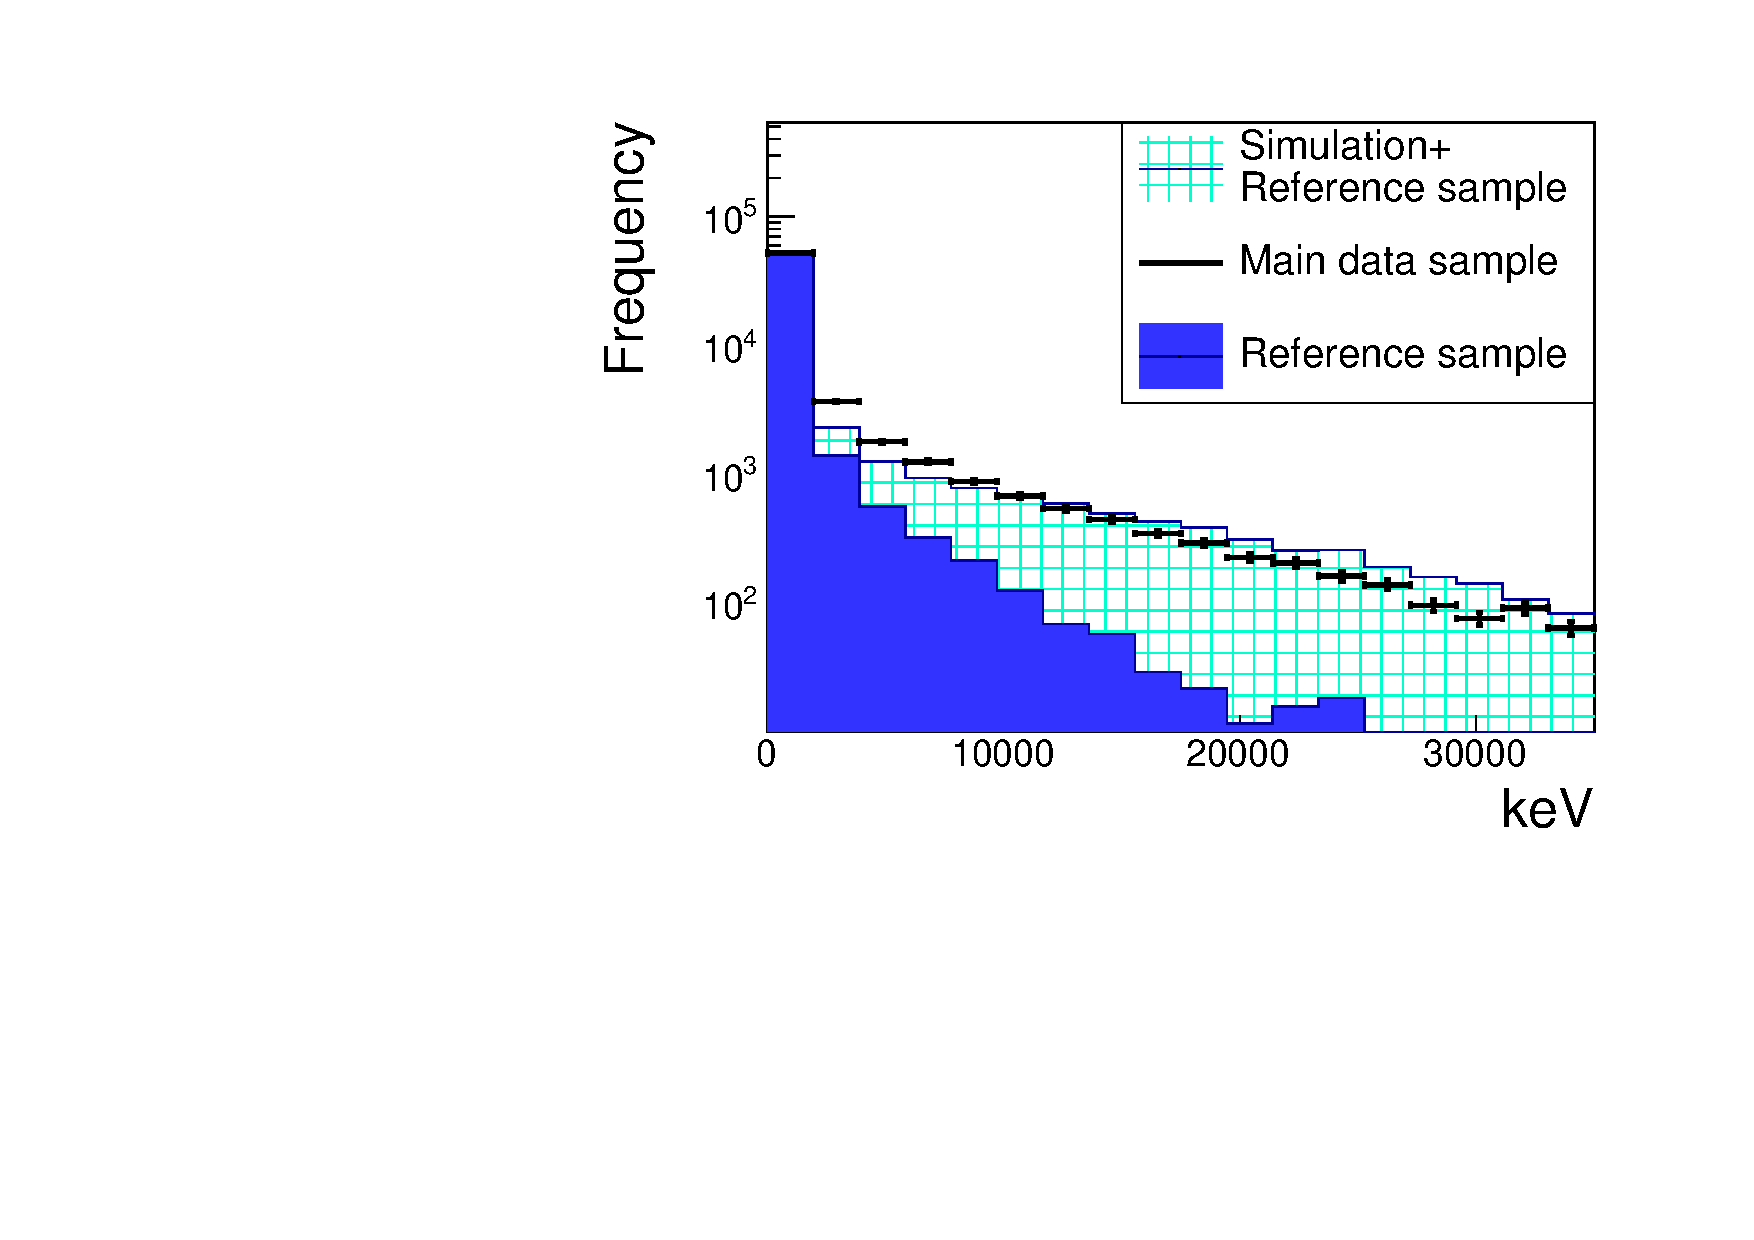
\includegraphics[width=3.55in]{fig/charge.pdf}
%%     \end{block}
%%   }
%%    \only<2>{\begin{block}{\centering Cluster energy in center}
%%     \centering
%%     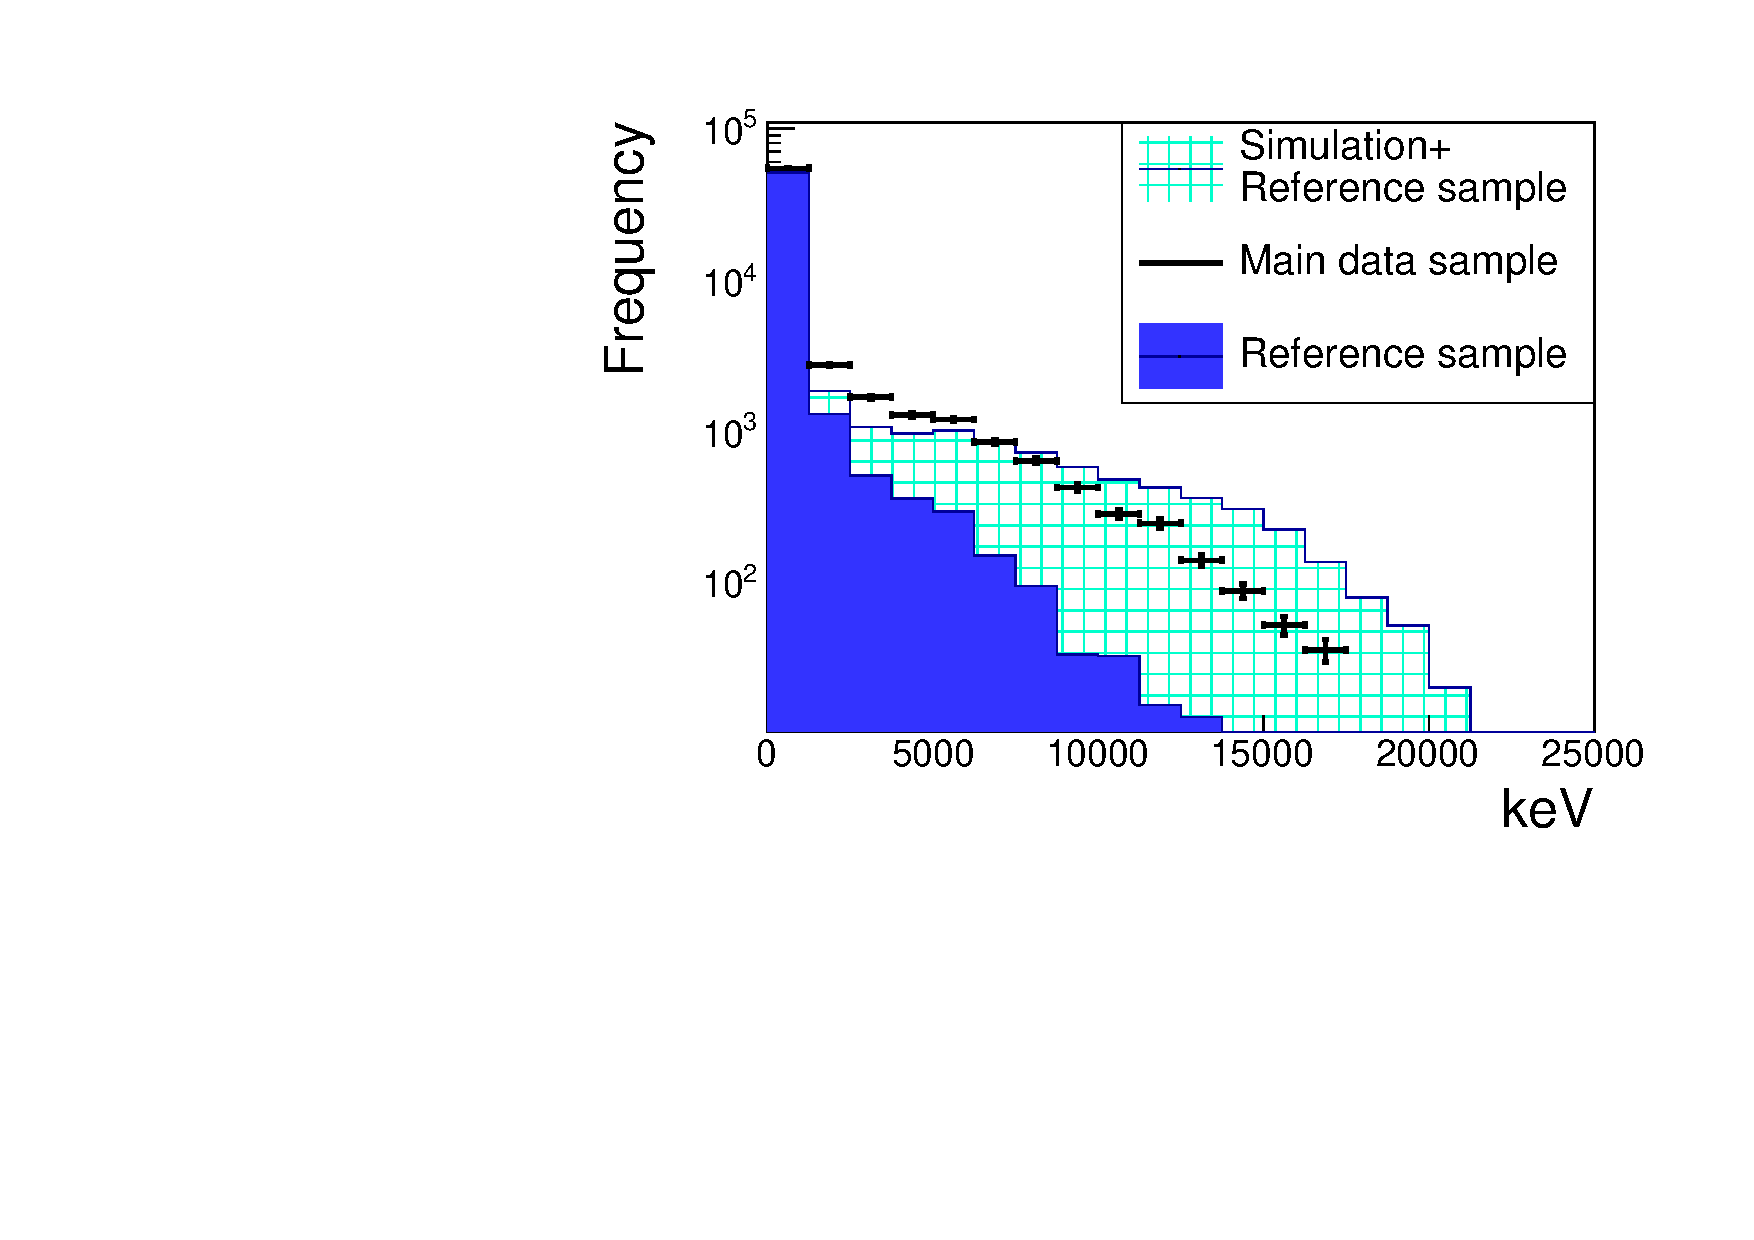
\includegraphics[width=3.55in]{fig/centerEnergy.pdf}
%%     \end{block}
%%    }
%%     \only<3>{\begin{block}{\centering Cluster size}
%%     \centering
%%     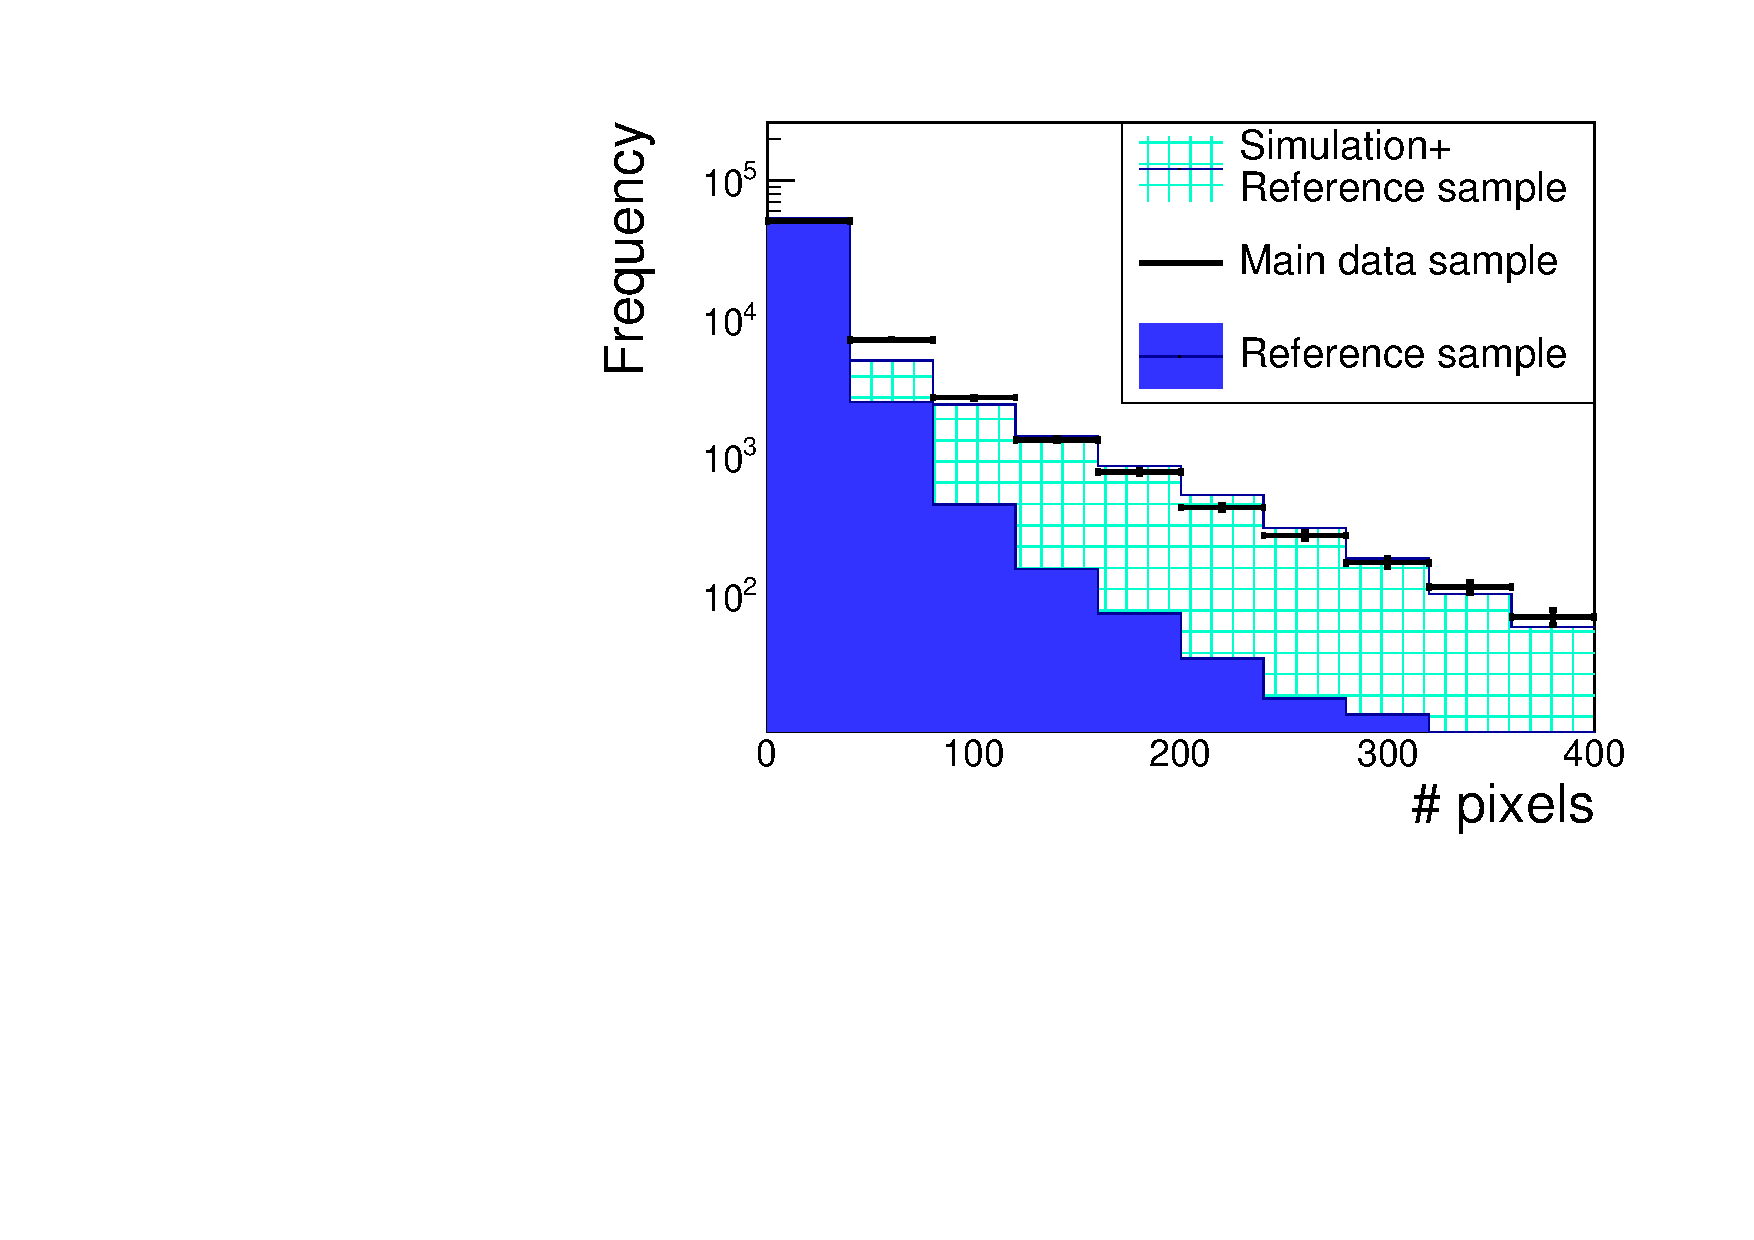
\includegraphics[width=3.55in]{fig/size.pdf}
%%     \end{block}
%%     }
%%      \only<4>{\begin{block}{\centering Number of prongs}
%%     \centering
%%     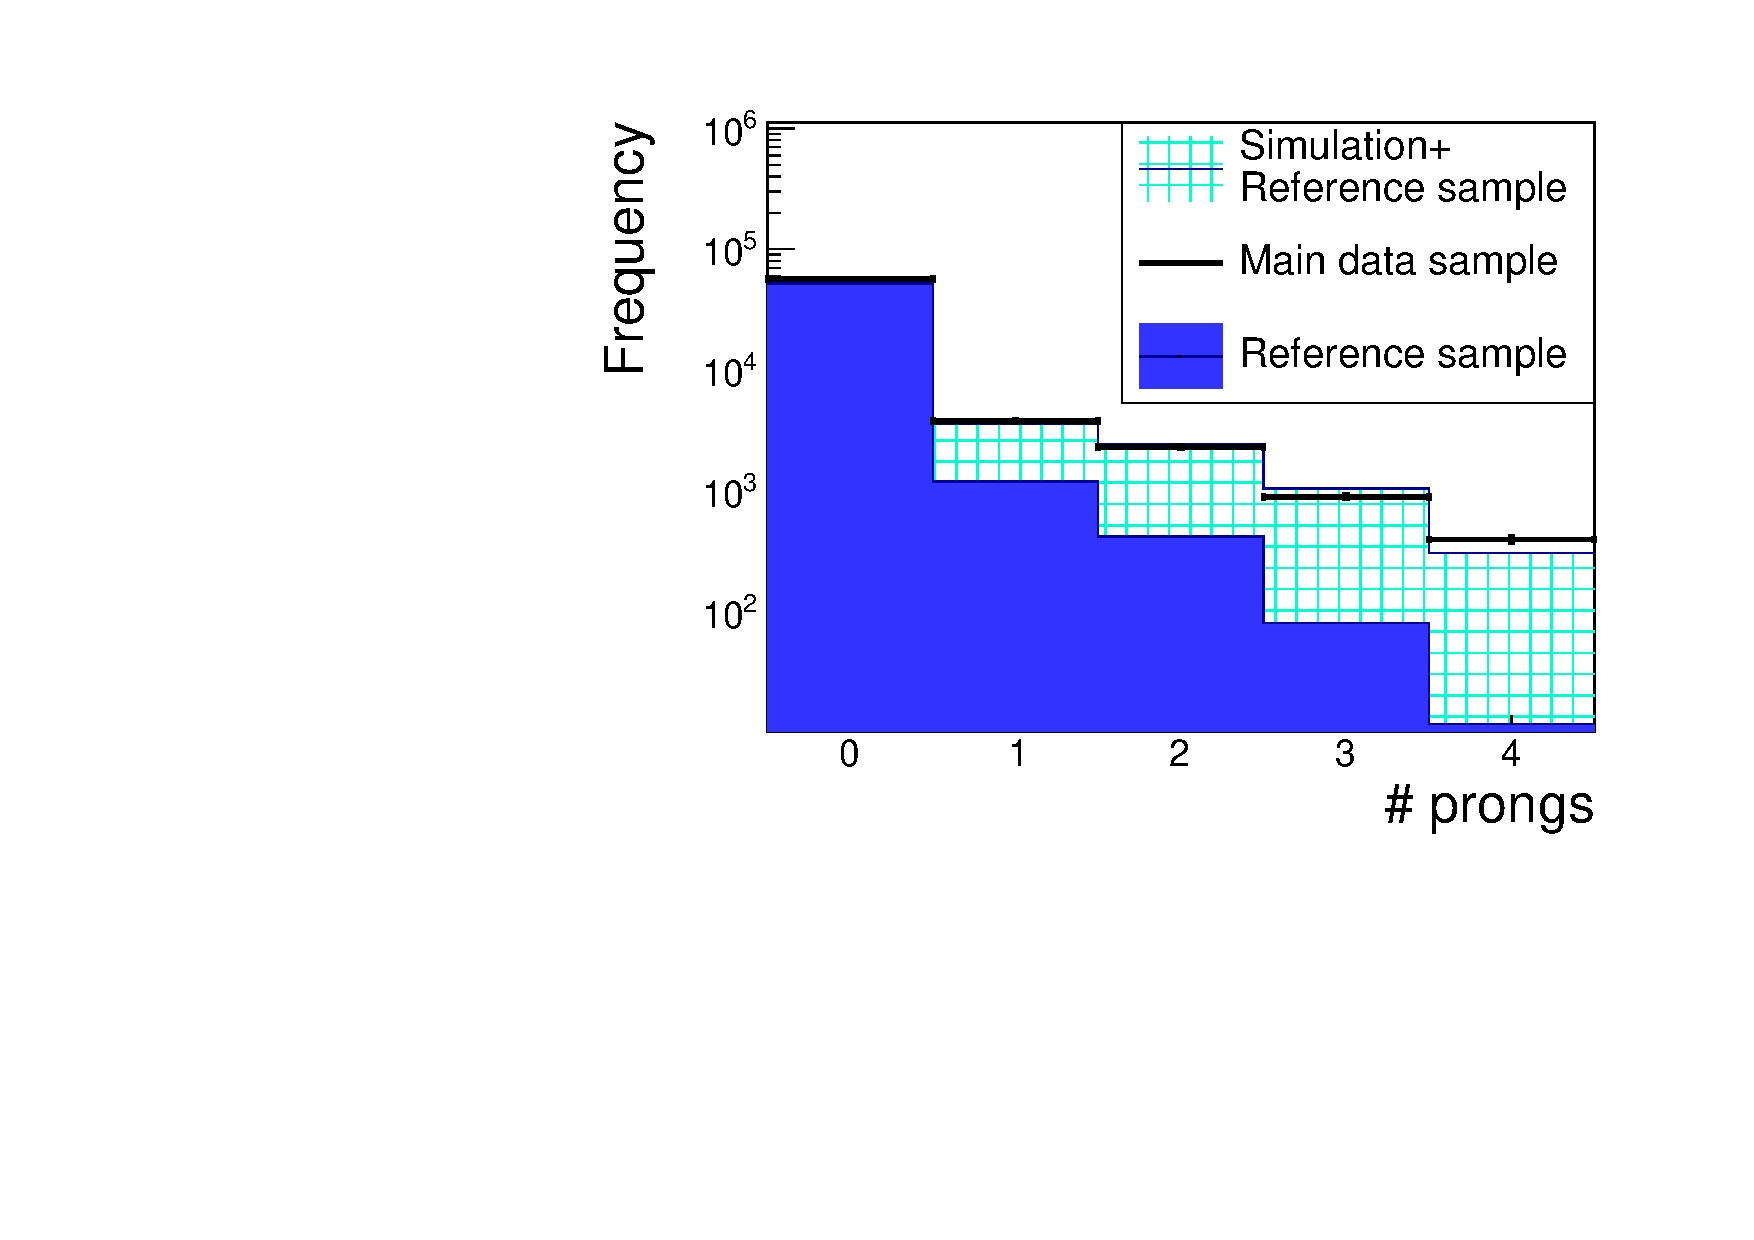
\includegraphics[width=3.55in]{fig/prongs.pdf}
%%     \end{block}
%%     }
%% \end{frame}



%% \begin{frame}{\centering Tagging efficiency}
%%   \begin{itemize}
%%   \item<1->{Anninhilation clusters are larger and have prongs}
%%   \item<2->{Trade off between tagging efficency and false positive rate}
%%   \uncover<3->{\item{A good compromise: At least 70 pixels and at least 1 prong}
%%     \begin{itemize}
%%     \item{Tagging efficency 50 $\pm$ 10\%}
%%     \item{Positive false rate below 1.1\%}
%%     \end{itemize}
%%     }
%%   \end{itemize}
%% \end{frame}


%% \begin{frame}{\centering Position resolution}
%%   \begin{columns}
%%     \begin{column}{0.5\textwidth}
%%       \begin{itemize}
%%       \uncover<1->{\item{Mass center method}
%%         \begin{itemize}
%%         \item{All clusters}
%%         \item{93~$\mu m$ resolution}
%%         \end{itemize}
%%         }
%%       \uncover<2->{\item{Vertex fitting method}
%%         \begin{itemize}
%%         \item{45\% of all clusters}
%%         \item{48~$\mu m$ resolution}
%%       \end{itemize}}
%%       \uncover<3->{
%%       \item{Vertex fitting method exluding bad fits}
%%         \begin{itemize}
%%         \item{22\% of all clusters}
%%         \item{22~$\mu m$ resolution}
%%       \end{itemize}}
%%       \item<4->{Change of annihilation fragments shown to have small effect on position resolution $ \approx \pm 1 \mu m$}
%%       \end{itemize}
%%     \end{column}
%%     \begin{column}{0.65\textwidth}
%%       \begin{figure}
%%         \begin{tikzpicture}
%%           \only<1>{\node at (0,0){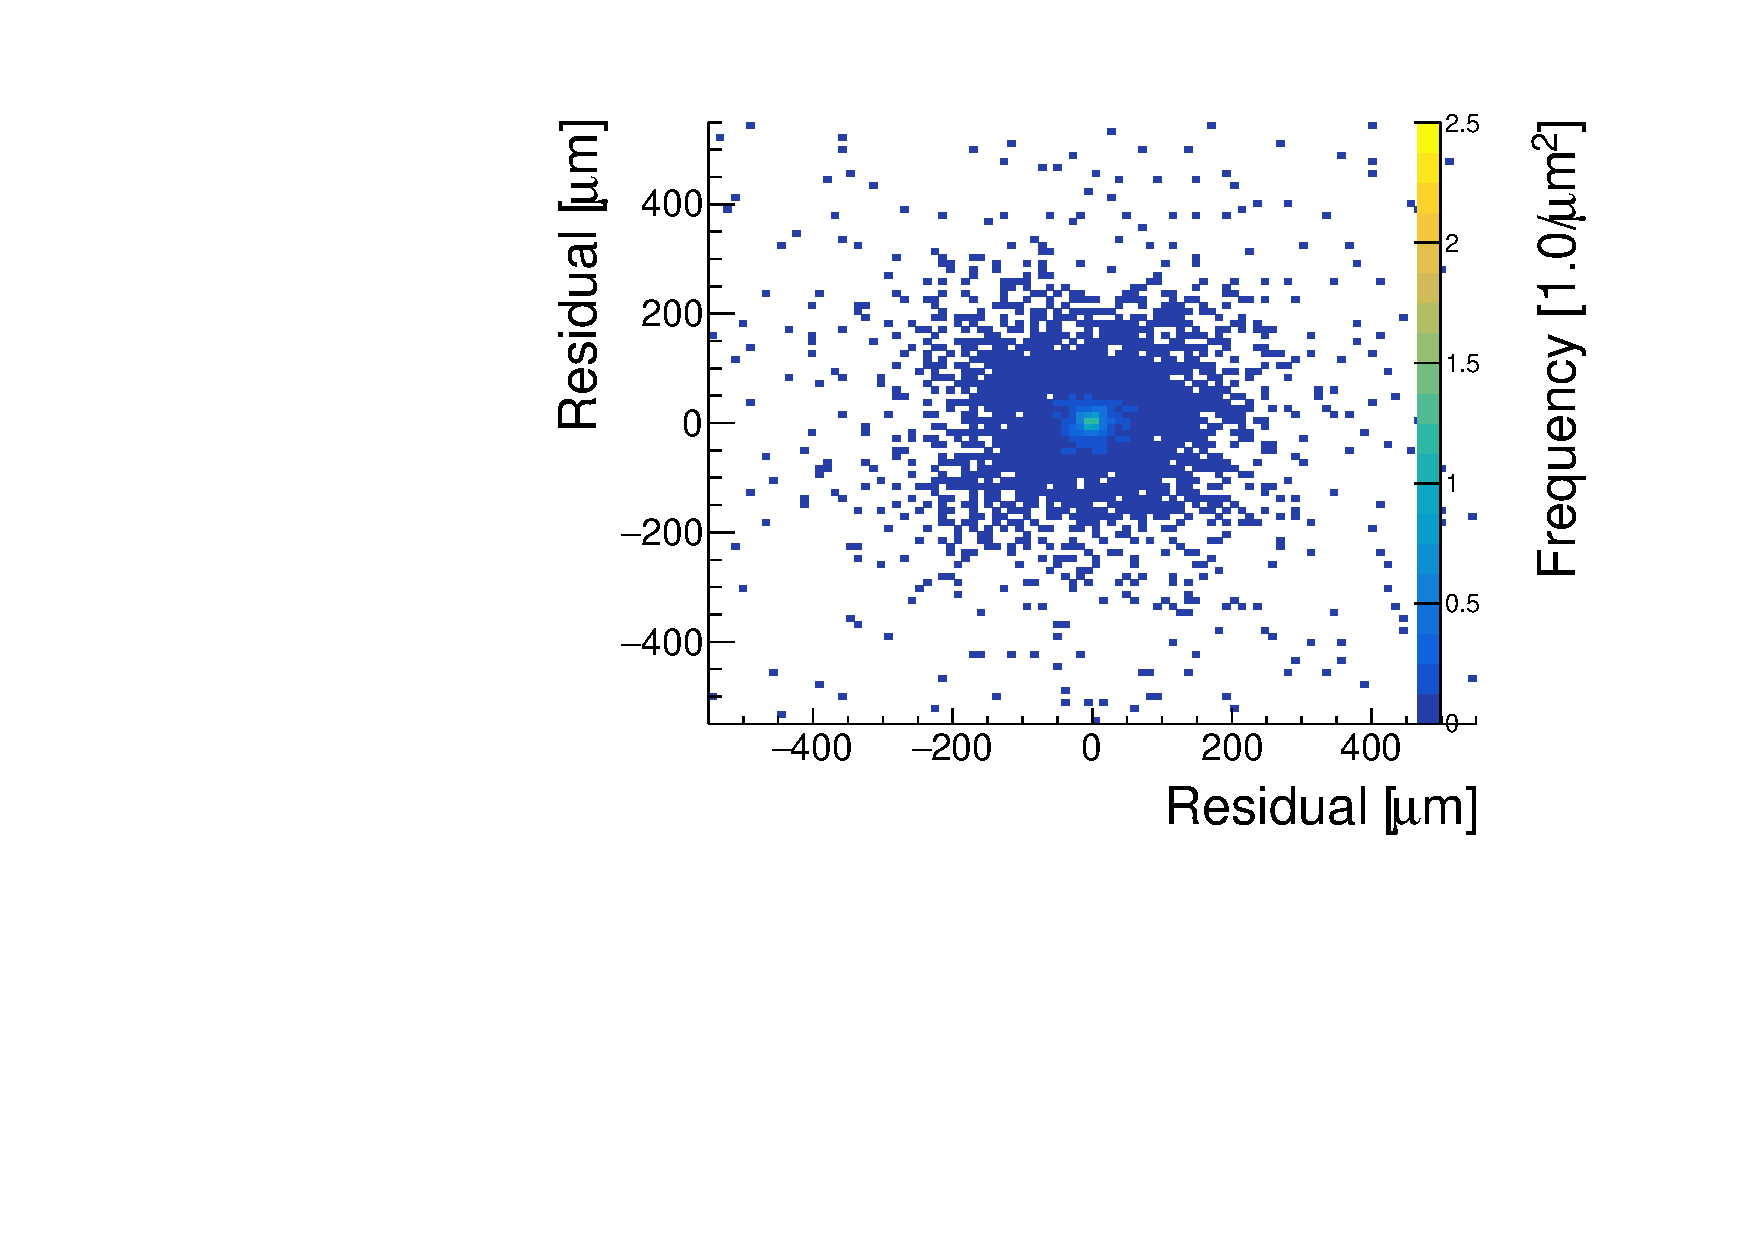
\includegraphics[width=\textwidth]{fig/2dfitSimple.pdf}};}
%%         \only<2>{\node at (0,0){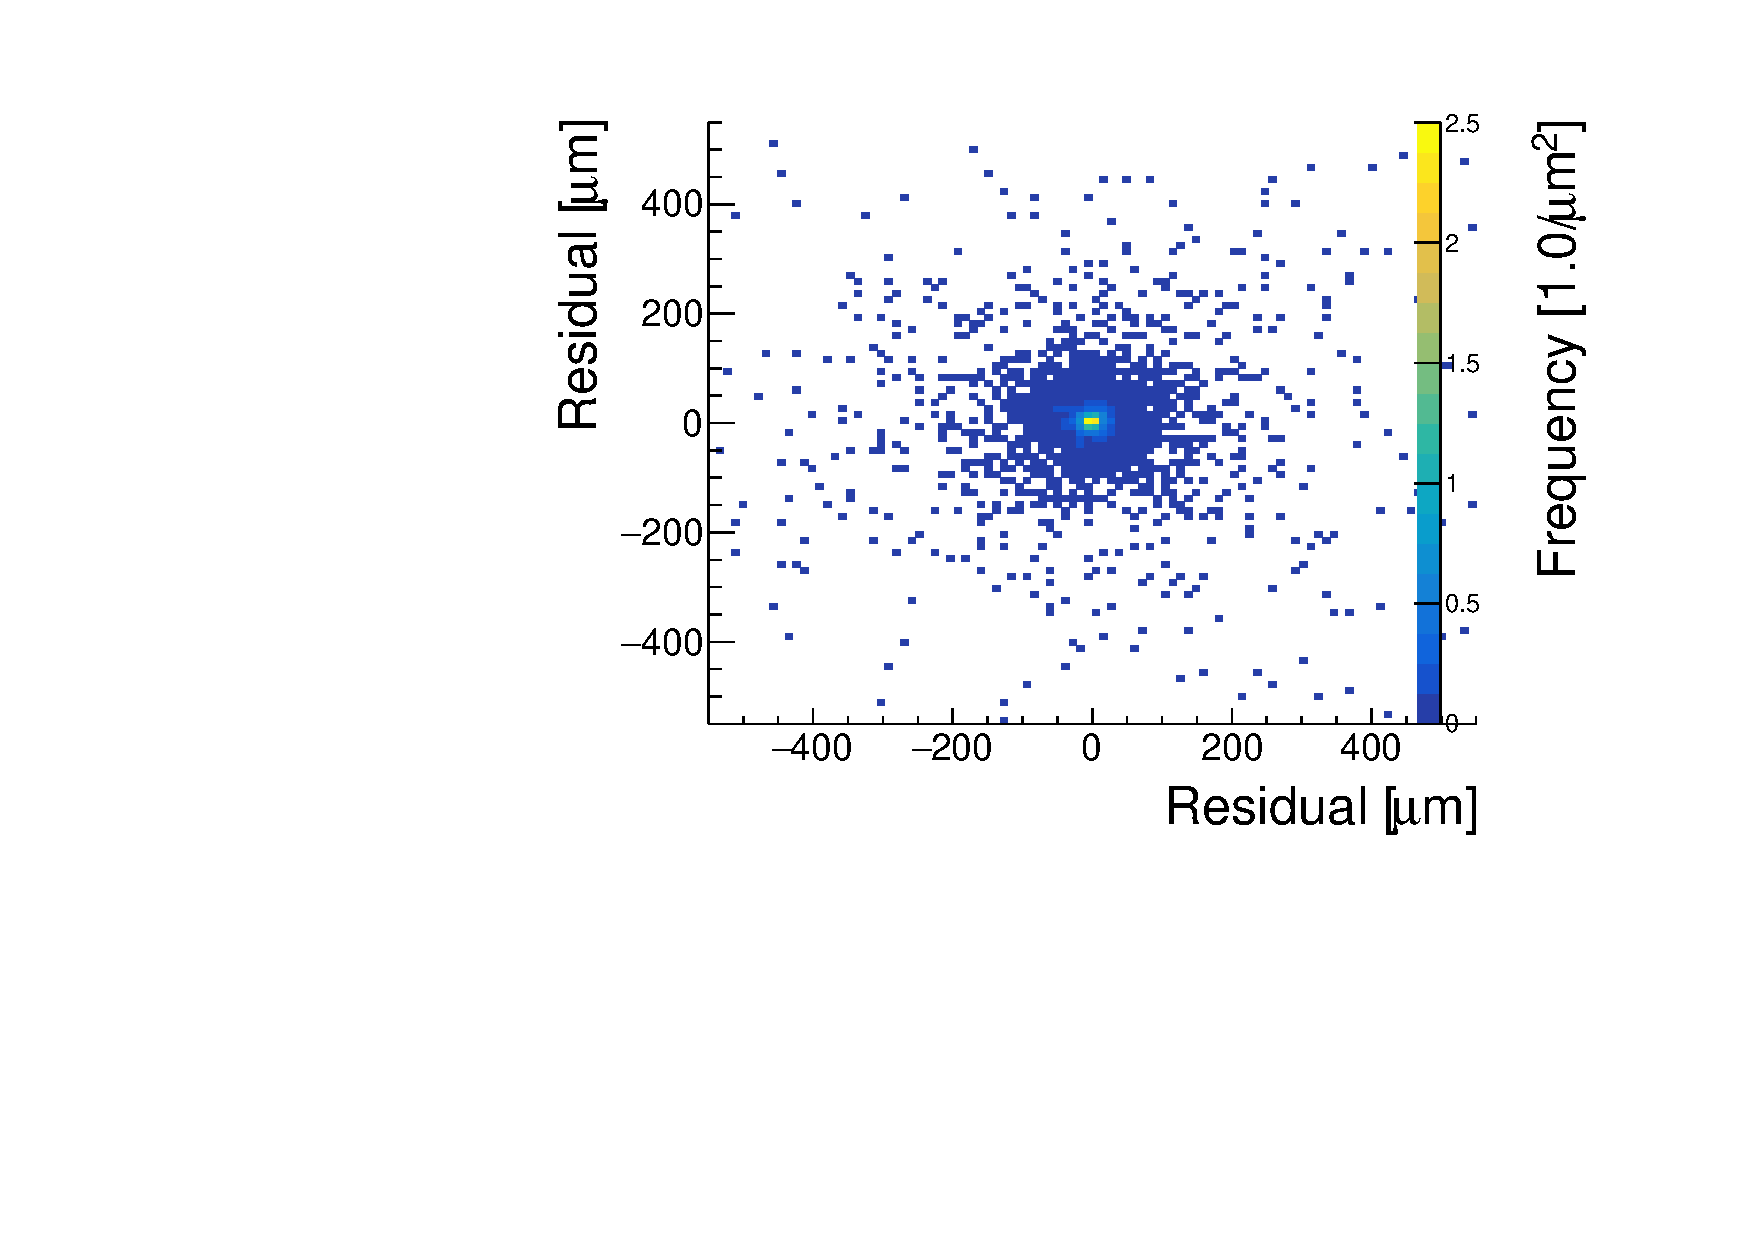
\includegraphics[width=\textwidth]{fig/2dfit.pdf}};}
%%         \only<3->{\node at (0,0){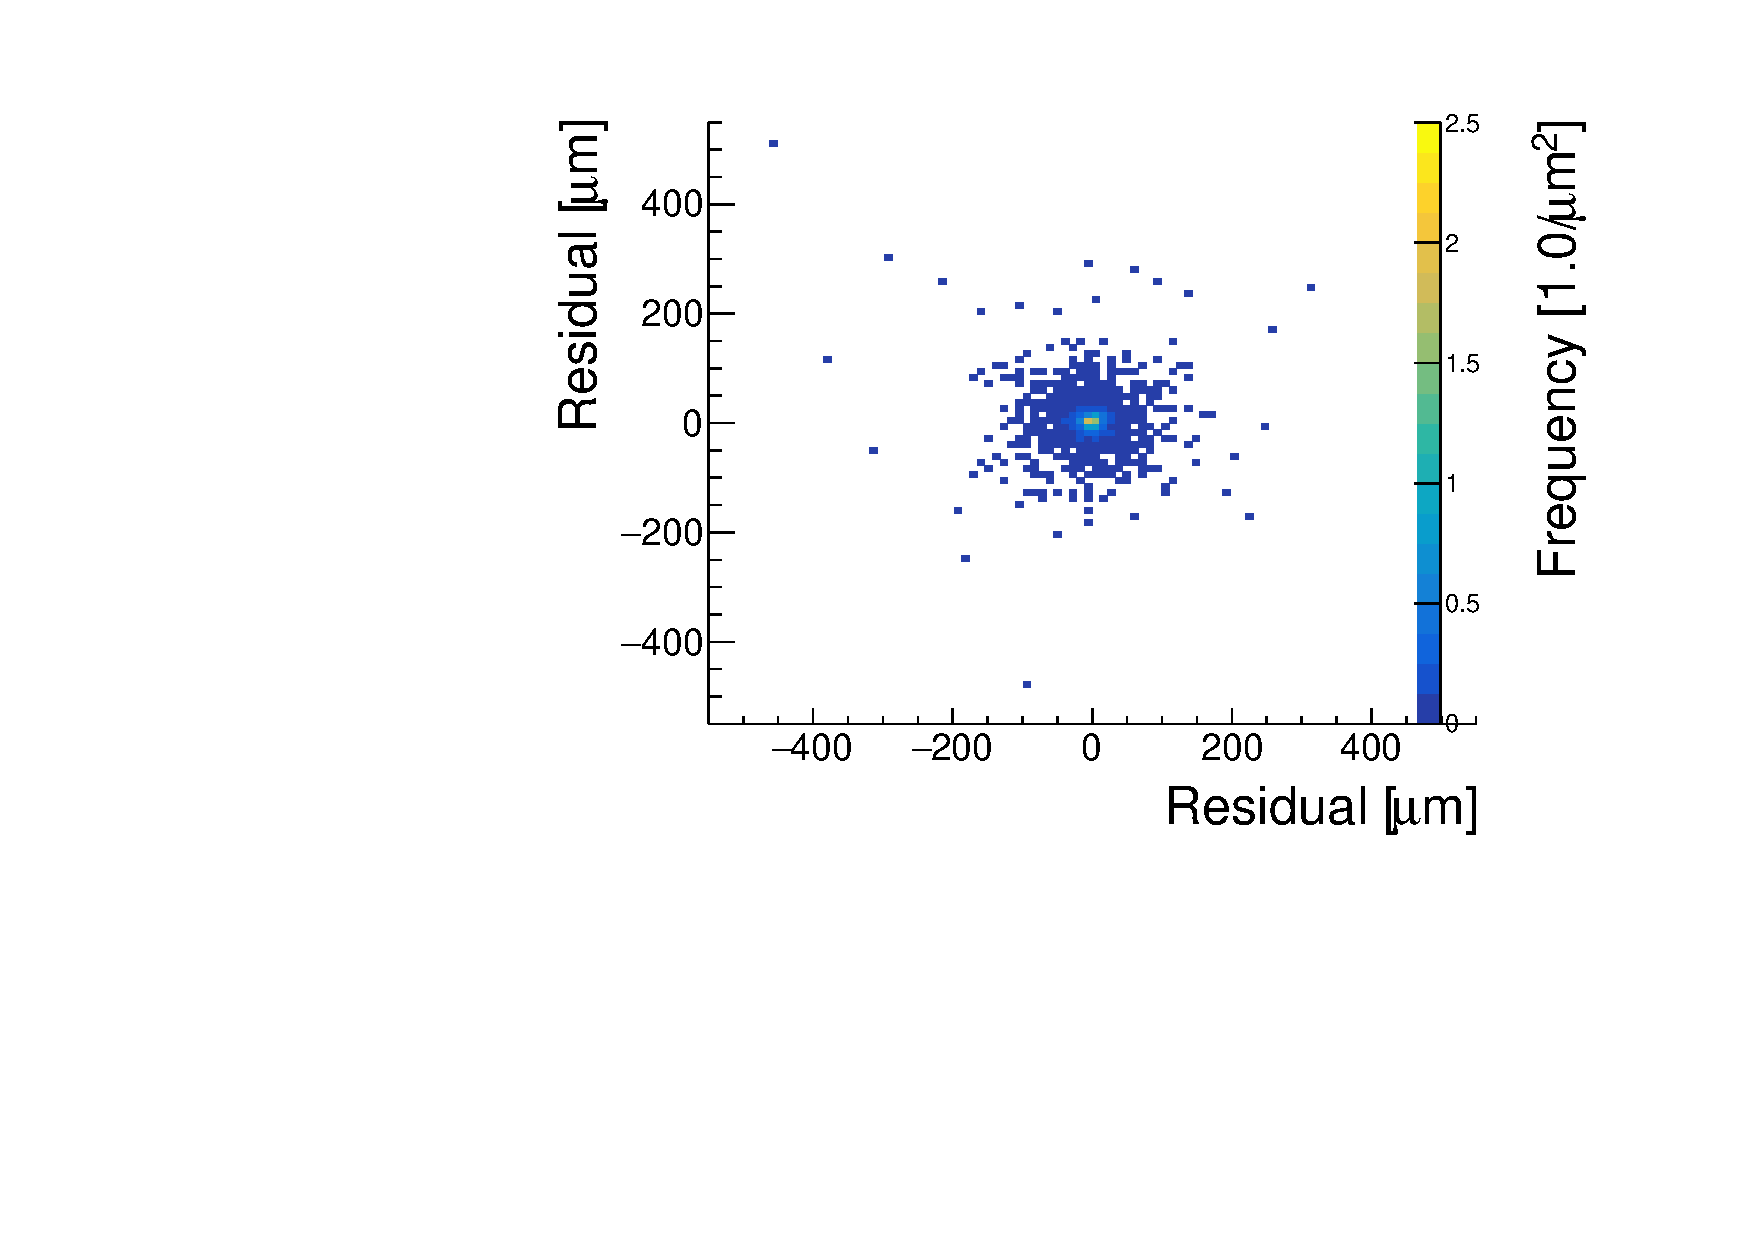
\includegraphics[width=\textwidth]{fig/2dfitSmall.pdf}};}
%%         \end{tikzpicture}
%%       \end{figure}
%%     \end{column}
%%   \end{columns}
%% \end{frame}



  
  
%% %%  % \only<1>{\begin{block}{\centering}
%% %%   \centering
%% %%     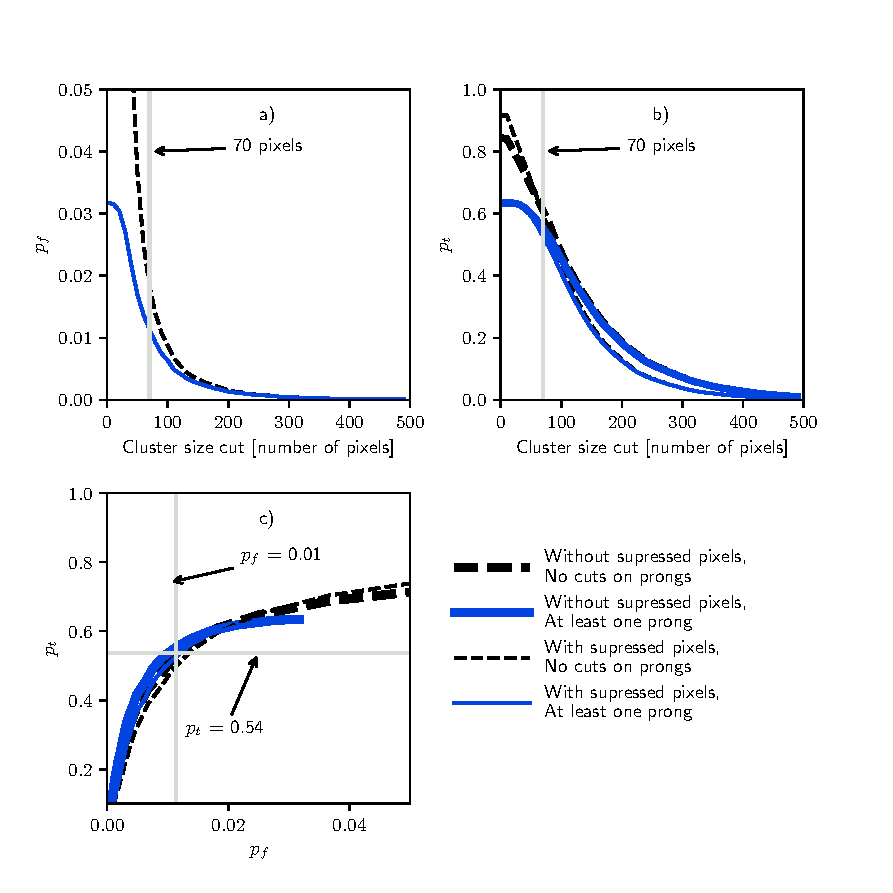
\includegraphics[width=3.17in]{fig/taggingEfficency}
%% %% %    \end{block}
%% %% %  }

%% \begin{frame}{Conclusion}
%%   \begin{itemize}
%%   \item{We can clearly see the annihilation clusters in the Timepix3}
%%   \item{Better understanding of annihilaitons in material}
%%    \item{Better understanding of for large energy depositions in the Timepix3 detector}
%%    \item{Detector response model taking into account th
%%      Developed a detector response model, and a full simulation of the GRACE beamline}
%%   \item{Tagging efficiency of 50~$\pm$~10\%}
%%   \item{False positive rate $< 1.0$\%}
%%   \item{Position resolution of 22~$\mu$m}
%%   \end{itemize}
%% \end{frame}
  


%% \begin{frame}{For more information}  
%%   \begin{block}{Find all the details here}
%%     \vspace{0.1cm}
%%   \emph{Antiproton tagging and vertex fitting in a Timepix3 detector”
%% S. Aghion et al 2018 JINST 13 P06004}
%%   \href{http://iopscience.iop.org/article/10.1088/1748-0221/13/06/P06004}{link}.\\
%%   \vspace{0.3cm}
%%   \href{https://github.com/helgaholmestad/finalTimepix}{https://github.com/helgaholmestad/finalTimepix}.
%%   \end{block}
%%   \end{frame}
%% \begin{frame}{Thank you and goodbye!!}
%%   %\begin{block}{}
%%   % \centering{
%%     %Jerome Alozy~~Xavi Cudie\\
%%     %Michael Campbel~~Lukas Tlustos}
%%   \begin{block}{
%%       \begin{columns}
%%         \begin{column}{0.5\textwidth}
%%           \begin{itemize}
%%             \setlength{\itemindent}{1.4cm}
%%           \item{Jerome Alozy}
%%           \item{Michael Campbell}
%%           \end{itemize}
%%         \end{column}
%%         \begin{column}{0.5\textwidth}
%%           \begin{itemize}
%%           \item{Xavi Cudie}
%%           \item{Lukas Tlustos}
%%           \end{itemize}
%%         \end{column}
%%       \end{columns}
%%     }
%%     \centering
%%     \vspace{0.5cm}
%%        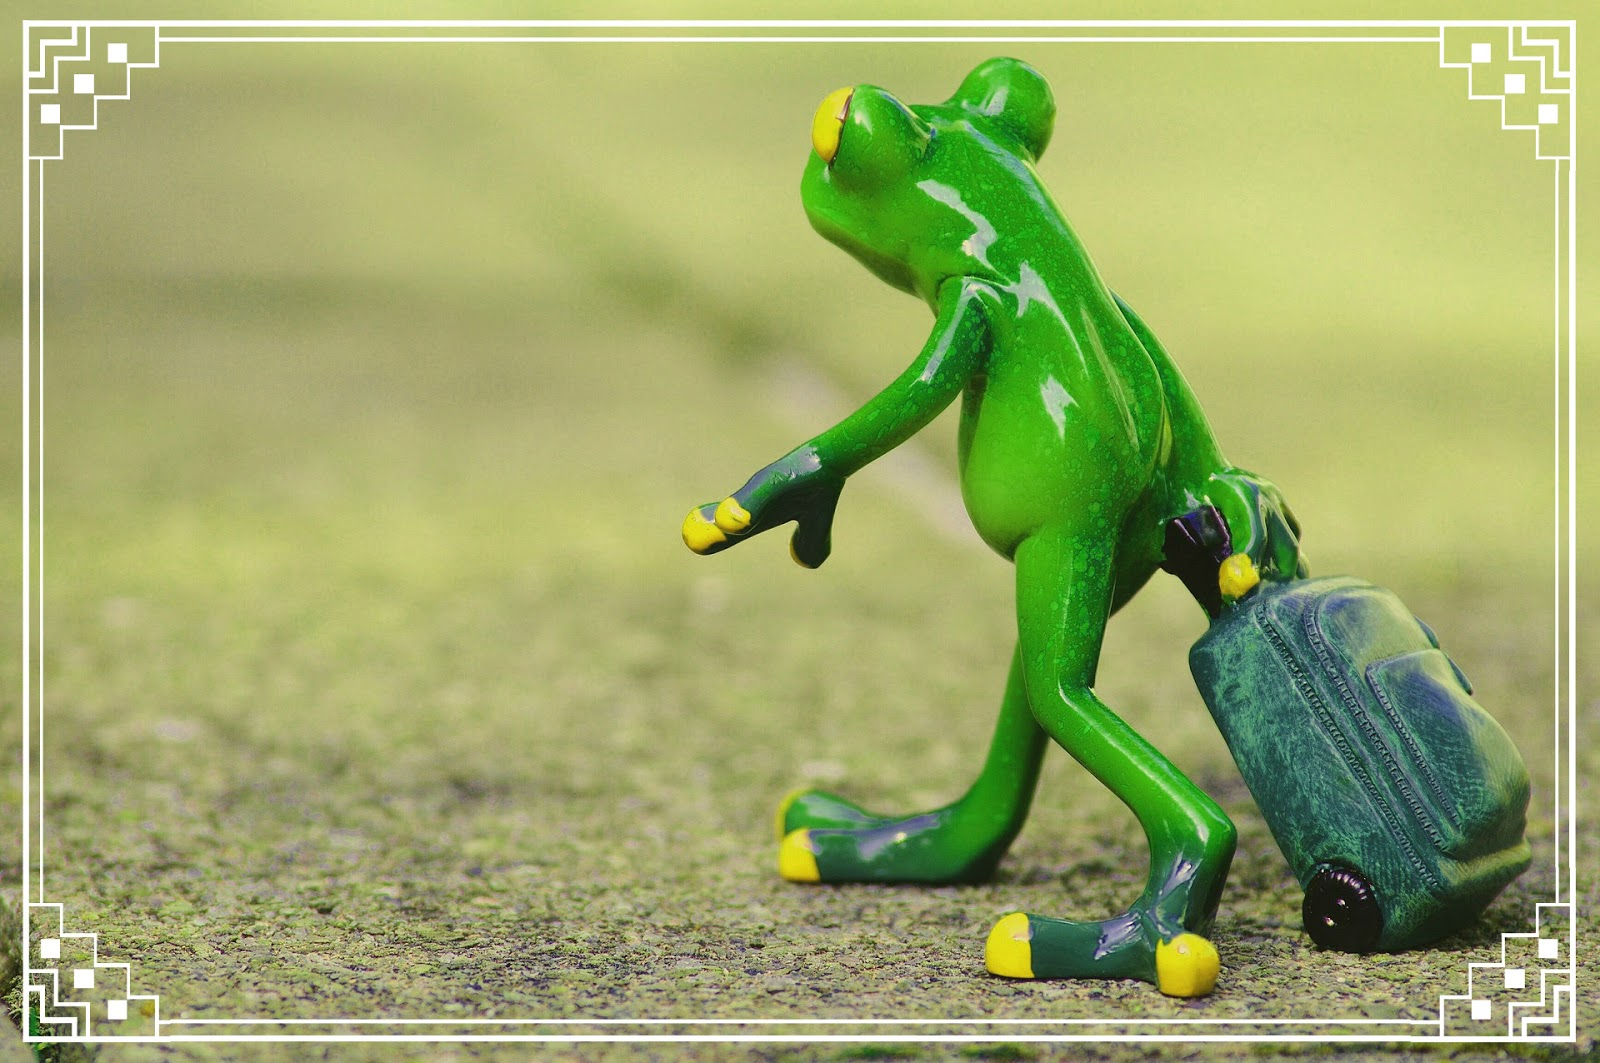
\includegraphics[width=3.00in]{fig/OnVacation.jpg}
%%   \end{block}
%%  %%  \begin{frame}{Thank you and goodbye!!}
%%  %%  %\begin{block}{}
%%  %%  % \centering{
%%  %%    %Jerome Alozy~~Xavi Cudie\\
%%  %%    %Michael Campbel~~Lukas Tlustos}
%%  %%  \begin{block}{\begin{itemize}
%%  %%        \setlength{\itemindent}{2.5cm}
%%  %%      \item{Jerome Alozy~~~~~~~~Xavi Cudie}
%%  %%      \item{Michael Campbell~~Lukas Tlustos}
%%  %%     \end{itemize}
%%  %%     }
%%  %%    \centering
%%  %%    \vspace{0.5cm}
%%  %%       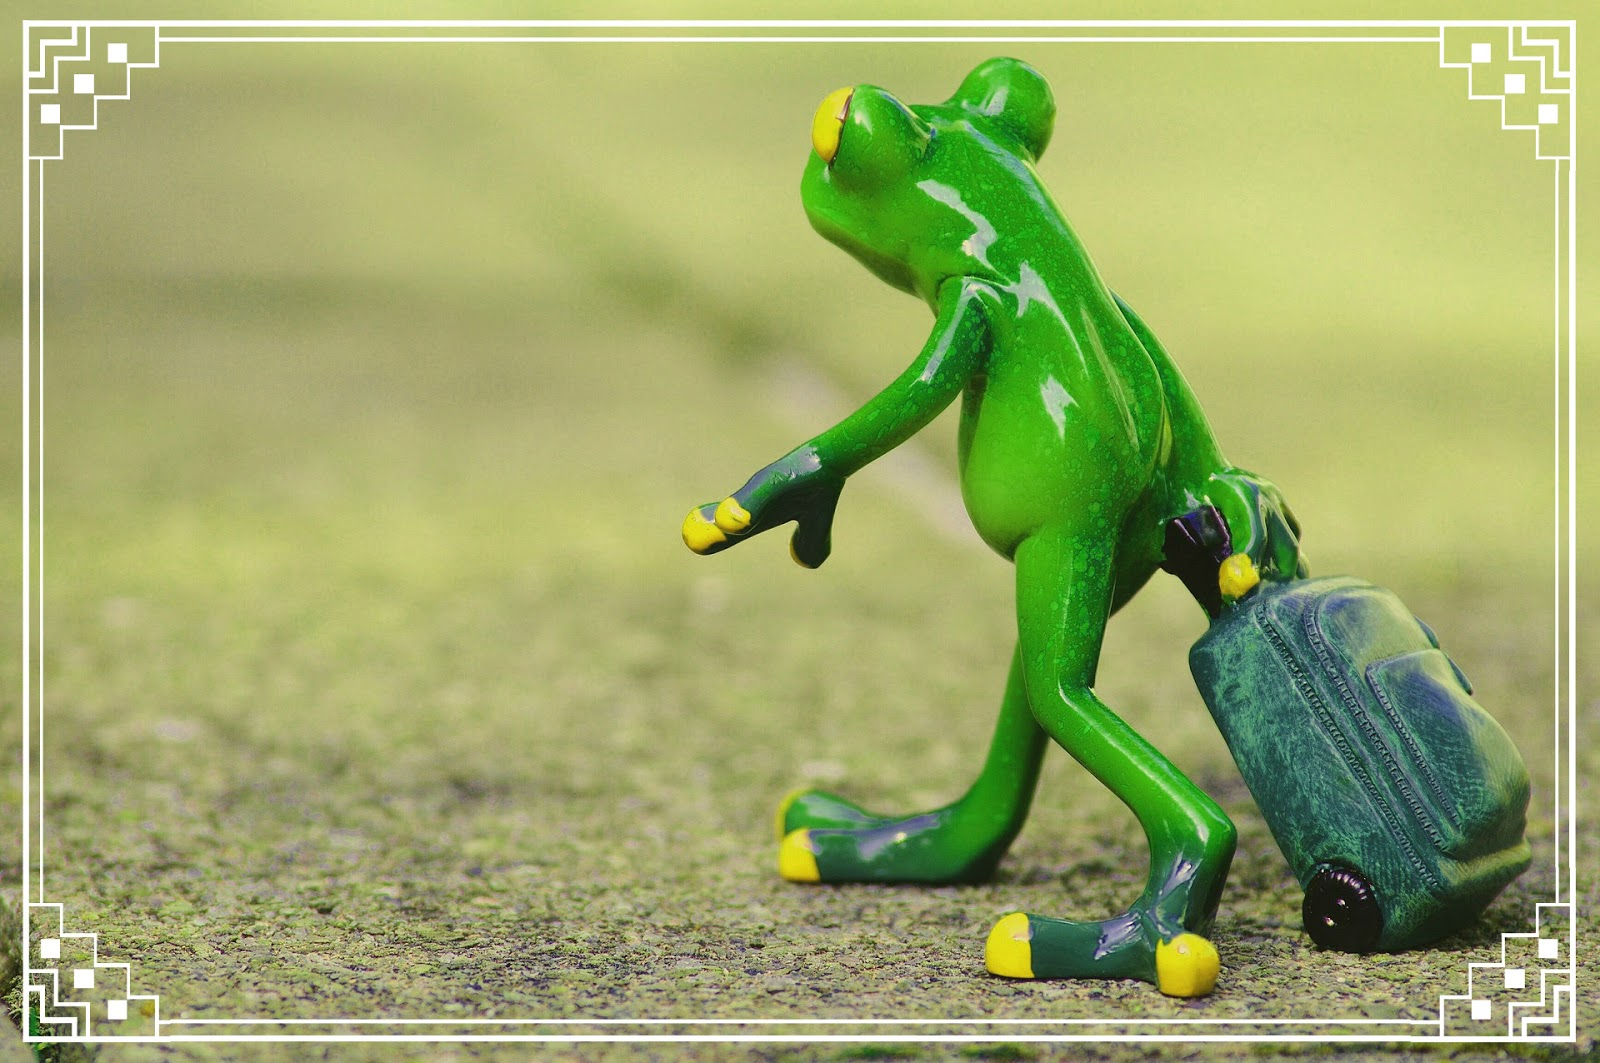
\includegraphics[width=3.00in]{fig/OnVacation.jpg}
%%  %% \end{block}
%% \end{frame}
\end{document}
